\documentclass[a4paper, 10pt]{article}
\usepackage[utf8]{inputenc}
\usepackage{verbatim}
\usepackage{listings}
\usepackage{graphicx}
\usepackage{a4wide}
\usepackage{color}
\usepackage{amsmath}
\usepackage{amssymb}
\usepackage[dvips]{epsfig}
\usepackage[toc,page]{appendix}
\usepackage[T1]{fontenc}
\usepackage{cite} % [2,3,4] --> [2--4]
\usepackage{shadow}
\usepackage{hyperref}
\usepackage{titling}
\usepackage{marvosym }
\usepackage{subcaption}
\usepackage[noabbrev]{cleveref}
\usepackage{wasysym}


\renewcommand{\topfraction}{.85}
\renewcommand{\bottomfraction}{.7}
\renewcommand{\textfraction}{.15}
\renewcommand{\floatpagefraction}{.66}
\renewcommand{\dbltopfraction}{.66}
\renewcommand{\dblfloatpagefraction}{.66}
\setcounter{topnumber}{9}
\setcounter{bottomnumber}{9}
\setcounter{totalnumber}{20}
\setcounter{dbltopnumber}{9}


\setlength{\droptitle}{-10em}   % This is your set screw

\setcounter{tocdepth}{2}

\lstset{language=c++}
\lstset{alsolanguage=[90]Fortran}
\lstset{basicstyle=\small}
\lstset{backgroundcolor=\color{white}}
\lstset{frame=single}
\lstset{stringstyle=\ttfamily}
\lstset{keywordstyle=\color{red}\bfseries}
\lstset{commentstyle=\itshape\color{blue}}
\lstset{showspaces=false}
\lstset{showstringspaces=false}
\lstset{showtabs=false}
\lstset{breaklines}
\title{FYS3150 - Project 5\\
Financial Modelling}
\author{Daniel Heinesen, Gunnar Lange}
\begin{document}
\maketitle
\begin{abstract}
We investigate a range of different models for the behavior of financial agents interacting with each other, aiming to extract an equilibrium distribution. We begin with a straightforwards Monte Carlo model, where two financial agents randomly split their wealth among each other. We expand this model by including the possibility of agents saving money, and by modifying the probability of an interaction by taking into account financial proximity and the effect of previous transactions. This is further developed by introducing some analytic solutions, to which we compare our simulations, and by an investigation into the way in which we can assert whether or not equilibrium has been reached. We find good agreement with analytic solutions where they exist. Our model behaves the way we expect for most parameters, but we observe some odd behavior for the case where previous transactions are significantly more important than financial proximity. All programs and plots employed in this article can be found on our \href{https://github.com/dulte/Comp-Phys/tree/master/Project5Final}{GIT-page}\footnote{https://github.com/dulte/Comp-Phys/tree/master/Project5Final}.
\end{abstract}
\tableofcontents
\section{Introduction}
Monte Carlo simulations of financial agents is at the core of the relatively new, interdisciplinary, field of econophysics. There has been a veritable landslide of such models presented in recent papers (see e.g. \cite{Self-adjusted}, \cite{Finite-size} or \cite{AgentBased}), ranging from simple models, where all agents have the same interaction probability and simply redistribute their money (see e.g. \cite{Gibbs}), to far more complex models including savings, financial proximity (see \cite{AgentBased} or psychological propinquity.\\
\linebreak
We present an overview of four models with varying degrees of complexity, in which we try to extract and understand the equilibrium distributions, as well as some some indicators of equilibrium. We begin with a theoretical overview of our four models, presenting the models, as well as some analytic solutions which exist for some of the models. We continue with a brief overview of our methods, including both how we implement the models and how we assess the equilibration point in our model. We then present our results and a discussion thereof.
\section{Theoretical model}
In this section we introduce the theoretical model necessary to model financial agents through Monte Carlo simulations. We also introduce some analytic solutions. 
\subsection{Simulating financial transactions}
We begin all our simulations with $N$ agents, each with a certain amount of wealth $m_i$, where $i \in [1, N]$.  For simplicity, we let all our agents begin with an equal amount of initial wealth, $m_i=m_j$ for $i,j \in [1,N]$. We subsequently let all agents interact with each other, according to four different set of rules, presented below. We let this interaction continue until equilibrium has been achieved, and we repeat these simulations until we have a sufficient amount of statistical data. The details of this last point are described in section \ref{Method_section}.
\subsubsection{Initial model for the interaction between two financial agents (model A)}\label{Initial_model}
We begin with a simple model for the interaction of two financial agents, as presented by \cite{Gibbs}. Assume that we, at random, pick two agents $i$ and $j$, each with wealth given by $m_i$ and $m_j$. We model the interaction between $m_i$ and $m_j$ as a complete, unbiased, exchange of wealth, that is; the agents combine their wealth, and then redistribute it by drawing a random number, $\epsilon$ $\in [0,1]$, from a uniform distribution, and then redistributing the wealth according to:
\begin{equation}
m_1'=\epsilon(m_1+m_2)
\end{equation}
\begin{equation}
m_2'=(1-\epsilon)(m_1+m_2)
\end{equation}
Where the primed quantities represent the wealth of each agent after the transaction. Notice that the total wealth is conserved in this interaction, seeing as:
$$m_1'+m_2'=\epsilon(m_1+m_2)+(1-\epsilon)(m_1+m_2)=m_1+m_2$$
Thus we are only redistributing wealth among our agents.
\subsubsection{First modification: Implementing savings (model B)}\label{Model_B}
We expand our model slightly by including the possibility of our agents retaining a certain amount of money in the transaction, as done by \cite{Gibbs}. This is modelled by a parameter $\lambda$, which describes the fraction of money saved by each agent. With this modification, we can rewrite the equations describing our interaction as:
\begin{equation}
\begin{split}
m_i'=\lambda m_i+\epsilon(1-\lambda)(m_i+m_j) \\
m_j'=\lambda m_j+(1-\epsilon)(1-\lambda)(m_i+m_j)
\end{split}
\end{equation}
Note that the total amount of wealth is still conserved, seeing as:
$$m_i'+m_j'=\lambda m_i+\epsilon(1-\lambda)(m_i+m_j)+\lambda m_j+(1-\epsilon)(1-\lambda)(m_i+m_j)=\lambda (m_i+m_j)+(1-\lambda)(m_i+m_j)=m_i+m_j$$
Thus we are still only redistributing wealth, but according to a different probability distribution. Note further that model A and model B are identical if $\lambda = 0$. We will let $\lambda \in [0, 0.25, 0.5, 0.9]$, and try to extract the behavior of the model for different $\lambda$. 
\subsubsection{Second modification: Including the effect of proximity (model C)}\label{Model_C}
Our second modification is inspired by a paper published by \cite{AgentBased}. Here, we introduce the possibility of two chosen agents not interacting at all, that is; we introduce a probability of interaction. We construct this probability in a biased way; making it more likely for agents with comparable amount of wealth to interact with each other. Specifically, we determine the probability of an interaction occurring between agents $i$ and $j$, $p_{ij}$, from the equation:
\begin{equation}\label{eq:Nearest_neighbors}
p_{ij}=2\left|\frac{m_i-m_j}{\langle m \rangle} \right|^{-\alpha} 
\end{equation}
Where $\alpha$ is a positive parameter which we vary and $\langle m \rangle$ is the mean wealth (which equals the initial wealth as we have a uniform initial distribution). Note that this differs slightly from the equation from \cite{AgentBased}, as they did not specify the initial wealth $m_0$. Note that equation \ref{eq:Nearest_neighbors} will give a qualitatively different behavior if the average monetary separation is large ($>>1$), than if it is small ($\simeq 1$). Therefore, we normalize this probability with the mean, to get an equation that is independent of the initial wealth. We also added an extra factor $2$. This results in more transactions occurring, which hopefully results in a faster onset of equilibrium. Note that \cite{AgentBased} simply stated that the probability is proportional to the quantity above, but did not specify a constant of proportionality. We choose, by trial and error, to let this constant be 2.\\
\linebreak
Whenever we have drawn two agents $i$ and $j,$ from our population, we also compute $p_{ij}$, and compare it to a random number, $\epsilon \in [0,1]$, drawn from a uniform distribution. If $\epsilon < p_{ij}$, the transaction occurs, otherwise, no transactions take place. We will implement this model with $\lambda=0$ (saving the full complexity to the last model), and letting $\alpha \in [0.5, 1.0, 1.5, 2.0]$. We try to extract the behavior of this model for different values of $\alpha$. 
\subsubsection{Final modification: Including the previous transactions (model D)}\label{Model_D}
Our final modification also originates from \cite{AgentBased}. Here, we include an "acquaintance factor", or a psychological propinquity, where the likelihood of a transaction occurring scales with the number of previous transactions between two agents $i$ and $j$. This is a simple modification of equation \ref{eq:Nearest_neighbors}, which we implement as:
\begin{equation}\label{eq:nearest_with_previous_transactions}
p_{ij}=2\left|\frac{m_i-m_j}{\langle m \rangle} \right|^{-\alpha}\left(\frac{c_{ij}+1}{\max_{i,j} (c_{ij})+1}\right)^{\gamma}
\end{equation} 
Where $c_{ij}$ is the number of previous interactions between agents $i$ and $j$ and $\gamma$ is a positive parameter which we vary. The additional $1$ is added to make it possible for agents that have not previously interacted to perform a transaction. Note that this model is initially identical to the model in equation \ref{eq:Nearest_neighbors}, but deviates at later times. Note further that this model also deviates slightly from the one presented by \cite{AgentBased}. There, it was not specified how to normalize the distribution, and therefore the probability will continuously increase, only ever reaching equilibrium when $p_{ij}=1$, $\forall i,j$, at which point it is equal to model A or B. We therefore hope that this modification will result in an earlier onset of equilibrium.
\subsection{Analytic solutions}\label{Analytic_solution}
In this section we present analytic solutions, wherever they are available. Model A and model B have analytic solutions, found in \cite{Gibbs} which we can use to test the consistency of our simulations directly. We also know approximately how we expect the tail of our other distributions (the richest agents) to behave.
\subsubsection{Analytic solution to the initial model (model A)}
The model from section \ref{Initial_model}, has an analytic solution which is described in detail by \cite{Gibbs}. There, it is shown that the equilibrium distribution of model A, in the continuous limit, approaches a Gibbs distribution of the form:
\begin{equation}\label{eq:Analytic_solution_A}
A(m)=\mu \exp(-\mu m)
\end{equation}
Where $\mu$ is a parameter which we have to determine. Note that, because $m$ (the amount of wealth) cannot be negative, this distribution is normalized\footnote{Because $\int_0^{\infty} \mu \exp(-\mu m)dm=1$}.
\subsubsection{Analytic solution to the first modification (model B) and variance}\label{variance}
The model from section \ref{Model_B} also has an analytic solution in the continuous limit. This is described in detail by \cite{Dynamics}. There it is shown that, if we normalize the wealth by its mean, i.e. let $\hat{m}=m/\langle m \rangle$, the probability distribution, $B(\hat{m})$, approaches:
\begin{equation}\label{eq:Analytic_solution_B}
B(\hat{m})=\frac{n^n}{\Gamma(n)}\hat{m}^{n-1}e^{-n\hat{m}}
\end{equation}
Where $n$ is given by:
$$n=1+\frac{3\lambda}{1-\lambda}$$
Note that this enables us to determine $\mu$ from equation \ref{eq:Analytic_solution_A} directly; as noted in section \ref{Model_B}, model A and model B are identical for $\lambda = 0$. Thus, we expect the analytic solution of model A to be given by:
\begin{equation}
A(\hat{m})=e^{-\hat{m}}
\end{equation}
We can also find an analytic expression for the variance of this distribution, which will be useful when investigating equilibrium, as described in section \ref{Method_section}. We begin with a general expression for a $\Gamma$-distribution:
\begin{equation}
B(m) = \frac{1}{\beta^{\alpha}\Gamma(\alpha)}m^{\alpha - 1}\exp\left(-\frac{m}{\beta}\right)
\end{equation}
This has a variance given by: 
\begin{equation}
V(m) = \alpha \beta^2
\end{equation}
If we use the analytic solution \ref{eq:Analytic_solution_B} we find:
\begin{equation}
\alpha = n
\end{equation}
\begin{equation}
\beta = \frac{1}{n}
\end{equation}
Thus we can now find an analytic variance for our distributions. For the distribution for model B:
\begin{equation}
V_B(m) = \left( 1 + \frac{3}{1-\lambda} \right) ^{-1}
\end{equation}
And for our distribution from model A:
\begin{equation}
V_A(m)=1
\end{equation}
\subsubsection{Consistency checks for all solutions}
For model C and D, we do not have analytic solutions readily available. However, as stated by \cite{Gibbs}, it is known from empirical studies that the richest agents in most society (the high-end tail of our distribution) tend to follow a Pareto distribution, given by:
\begin{equation}\label{eq:Anayltic_solution_C_D}
C(m) \propto m^{-1-\beta}
\end{equation}
Where $\beta \in [1,2]$. Thus, we can check how realistic our models are, by fitting a function of the form given in equation \ref{eq:Anayltic_solution_C_D} to the tail of our distribution, to see whether or not the richest agents follow the empirical Pareto distribution. This can be done for all models, to assess whether or not they represent a realistic economy.
\section{Methods}\label{Method_section}
Here, we introduce the methods that we employ to ensure that we get sufficient, reliable, statistical data, as well as some technicalities relating to our numeric implementation of the models discussed in the previous section.
\subsection{Obtaining reliable data}
We only want to analyze steady-state distributions, where the final distribution stays approximately constant. Note that, due to the dynamic nature of our system, the distribution at any specific instance may vary quite substantially, even at equilibrium. Thus, extracting a single distribution after a given number of transactions will give rise to significant statistical uncertainty. Therefore, we perform many repetitions of each experiment, starting with the same initial configuration, and then average the distributions that we extract. We will refer to each such repetitions, consisting of a given number of transactions, as a Monte Carlo cycle.\\
\linebreak
Whether or not we get reliable results will therefore hinge on two criteria:
\begin{itemize}
\item Having a sufficient number of transactions per Monte Carlo cycle
\item Having a sufficient number of Monte Carlo cycles
\end{itemize}
We need to have enough transactions per Monte Carlo cycle for the system to "forget" its initial state - that is, we need to have enough transactions to ensure that we have achieved equilibrium in the system. As discussed above, however, the distribution from a single cycle, even at equilibrium, is prone to statistical fluctuations. Thus, to get reliable data, we will have to perform sufficient Monte Carlo cycles for the distribution to stabilizes.\\
\subsubsection{Ensuring we perform a sufficient number of transactions}
A simple, yet efficient, way to investigate the number of transactions that we require, is to write out the variance of our distribution as a function of the number of transactions for a single Monte Carlo cycle. We compute the variance of the distribution as:
\begin{equation}
\mathrm{Var}_k(x)=\frac{\langle m^2 \rangle - \langle m \rangle^2 }{k}
\end{equation}
Where $\langle m \rangle$ denotes the mean of the distribution of wealth (which in our case is always the initial amount of wealth, as we start with a uniform distribution) and $k$ is the number of performed transactions.\\
\linebreak
Because we start with a uniform distribution of wealth, the variance will start out at zero. We expect it to subsequently increase with more transactions and finally to stabilizes, fluctuating around some value. We determine the required number of transactions to be the point where the variance stabilizes.
\subsubsection{Determining the number of Monte Carlo cycles needed}
We determine the number of Monte Carlo cycles needed by looking at the difference in the average of the distribution between two subsequent Monte Carlo cycles. We calculate this relative difference as:
\begin{equation}\label{eq:Relative_diff_MC_steps}
\delta = \frac{|\vec{M}_{i}-\vec{M}_{i-1}|}{|\vec{M}_i|}
\end{equation}
Where $\vec{M}$ is a vector with $N$ components, containing the wealth of each agent. $M_i$ represents the \textit{average wealth} after $i$ Monte Carlo cycles (i.e. the average of the distributions from all previous Monte Carlo cycles), and $M_{i+1}$ represents the same average, but with an additional Monte Carlo cycle taken into account. We expect $\delta$ to approach zero as the number of Monte Carlo cycles increases, as the statistical fluctuations from each cycles cancel each other out for a sufficiently large number of cycles. Notice, however, that additional Monte Carlo cycles incur additional computation time, which quickly racks up. Therefore, we choose a number of Monte Carlo cycles which balances computational feasibility with a sufficiently low $\delta$. 
\subsection{Normalizing the data}
We normalize all our data, so that they represent probability distributions. This is done by dividing the wealth of every player by the mean wealth, $\langle m \rangle$. 
\subsection{Determining the number of bins}
We chose a bin resolution of $0.02 \cdot N$. In order for the computations to be feasible, we require a maximum boundary for the highest bin. As the variance of the distributions varies with $\lambda$ , we implement an upper bound that depends upon $\lambda$. We chose:
\begin{equation}\label{eq:M_max}
m_{max} = \frac{2\langle m \rangle}{\sqrt{\lambda + 0.1}} + \chi
\end{equation}
$\chi$ is a number that we employ when we want to look at the tail. When we want to look at the tail, we have to ensure to include the few agents with a lot of money. With $\chi = \langle m \rangle$ it can be shown that
\begin{equation}
\min[B(m\leq m_{max},\lambda)] = \int_0^{m_{max}} \frac{n^n}{\Gamma(n)}m^{n-1}\exp(-nm) = 0.999636 
\end{equation}
Thus we except to include $99.9636 \%$ of the agents when looking at the tail. \\
\linebreak
When not looking at the tail, we let $\chi = 0$. Then we expect to include $99.19\%$ of the agents. This was employed in order to reduce the runtime. \\
\linebreak
We then divide the interval $(0,m_{\max})$ into bins of size $0.02$, and for each Monte Carlo cycle we update the distribution.
\subsection{Determining the Tail}\label{Tail_section}
We used $m_{\max}$ from equation \ref{eq:M_max} to determine the size of the tail. We defined the tail as the interval $(m_{max},m_{max}+\langle m \rangle)$, where we have set $\chi=0$ at the left end point. We expect this interval to include $8 \permil$ of the agents. Not all distributions fitted well into this interval, however, and the lower bound was lowered somewhat for higher values of $\lambda$.
\subsection{Implementing the Monte Carlo simulations}
As the main algorithm for simulating the transactions is relatively short, we present, in Pseudo-Code, the program for computing model A below:
\lstinputlisting{Pseudo_code_simple_walkers.cpp}
Note that the other models can be easily implemented by expanding the loop over transactions slightly.
\pagebreak



\section{Results and discussion}
\subsection{Results from the initial model (model A)}
\subsubsection{Results from our investigation into the optimal combination of parameters}
The results from our investigation into the optimal parameters for model A are shown below:
\begin{figure}[!ht]
    \centering
    \begin{subfigure}[H!]{0.5\textwidth}
        \centering
        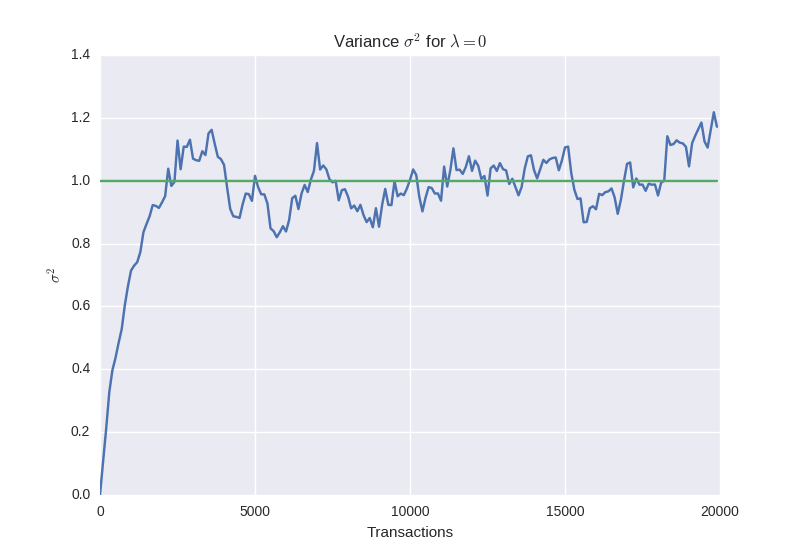
\includegraphics[height=2.0in]{varLamb0.png}
        \caption{The variance of a single Monte Carlo cycle}\label{fig:ModelA_Var}
    \end{subfigure}%
    ~ 
    \begin{subfigure}[H!]{0.5\textwidth}
        \centering
        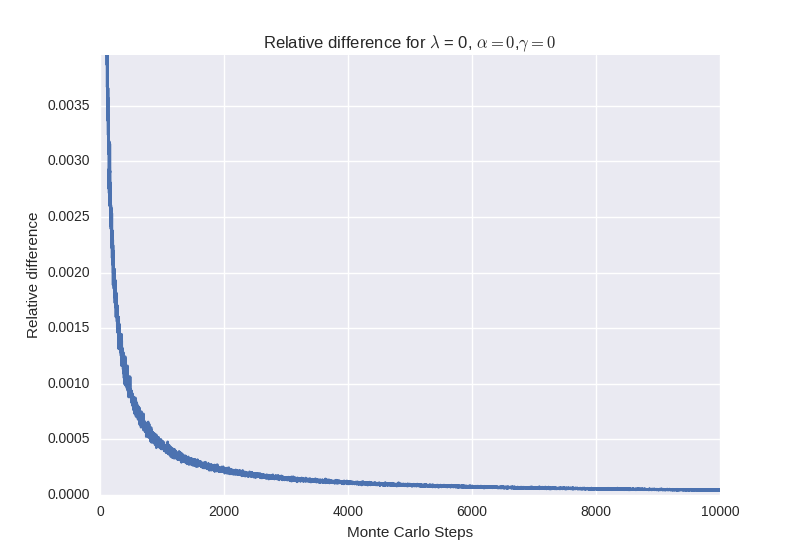
\includegraphics[height=2.0in]{relDiffL0A0G0.png}
        \caption{The difference in the distribution for successive Monte Carlo cycles}\label{fig:ModelA_MC_steps}
    \end{subfigure}
    \caption{Plots from our investigation into the optimal choice of parameters. Figure \ref{fig:ModelA_Var} shows how the variance of our distribution evolves with the number of transactions. This is for a single Monte Carlo cycle, with $N=500$ agents, and the initial wealth, $m_0=1000$. In figure \ref{fig:ModelA_MC_steps}, we show how the difference between successive average distributions evolves with the number of Monte Carlo steps. Each Monte Carlo cycle consists of $10^4$ transactions. Note that the $x$-axis does not start at zero, for a better graphical presentation of the long-term development. The analytic variance is from section \ref{variance}}\label{fig:ModelA}
\end{figure}
\subsubsection{The distribution from model A}
We discuss later how we decide on a combination of parameters. We present the final, average, distribution, for this combination of parameters, below:\\
\linebreak
\begin{figure}[!hb]
\centering
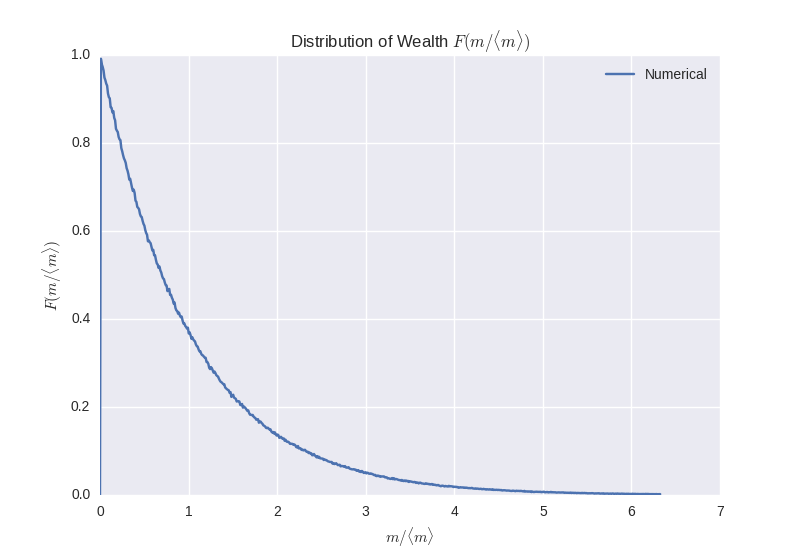
\includegraphics[height=2.0in]{distLamb0.png}
\caption{The final distribution of wealth from model A. Here $\langle m \rangle$ is the average wealth, which equals the initial wealth per agent, $m_0=1000$. This simulation was run with $500$ agents, performing $10^4$ transactions per Monte Carlo cycles, with a total of $10^4$ Monte Carlo cycles.}\label{fig:ModelA_final_distribution}
\end{figure}
\newpage
\subsubsection{Comparison with the analytic model}
We also include a logarithmic plot, of the above distribution, together with the analytic solution from section \ref{Analytic_solution}, to investigate how well our numerical distribution fits our analytic model.
\begin{figure}[!ht]
    \centering
    \begin{subfigure}[H!]{0.5\textwidth}
        \centering
        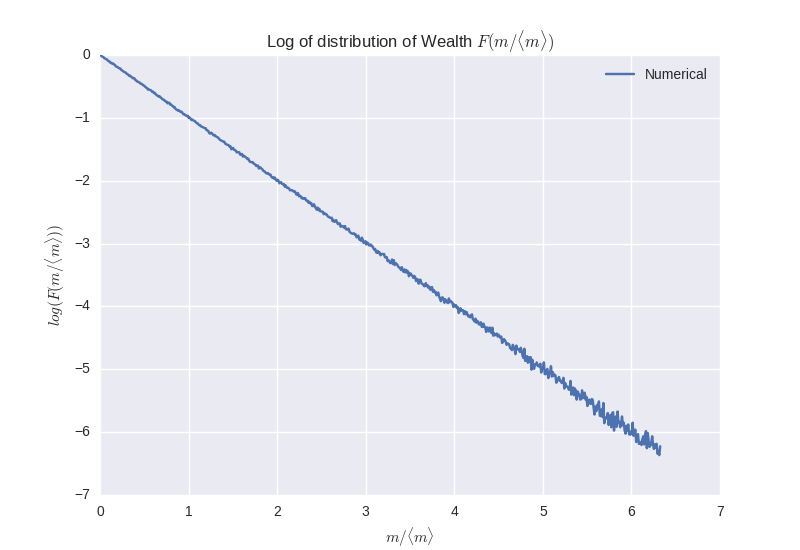
\includegraphics[height=2.0in]{logDistLamb0.png}
        \caption{A logarithmic plot of figure \ref{fig:ModelA}}\label{fig:ModelA_log_raw}
    \end{subfigure}%
    ~ 
    \begin{subfigure}[H!]{0.5\textwidth}
        \centering
        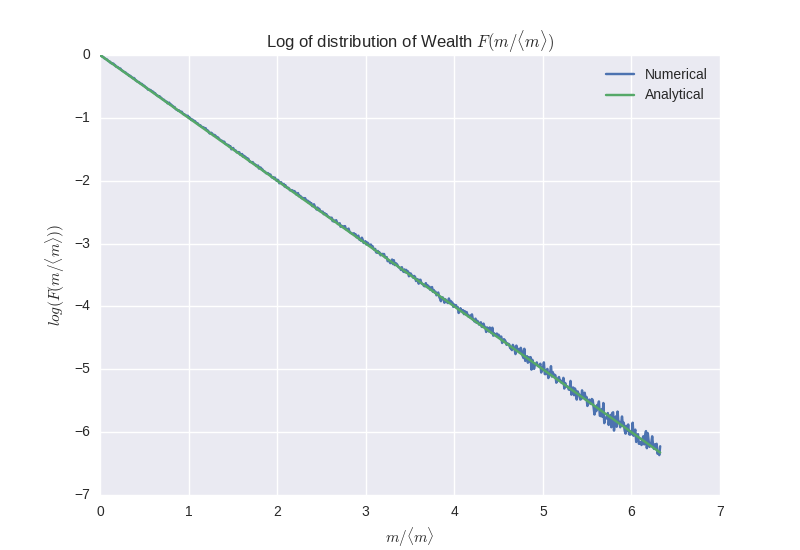
\includegraphics[height=2.0in]{logDistLamb0WAnalyt.png}
        \caption{The same plot, with analytic solution}\label{fig:ModelA_log_fit}
    \end{subfigure}
    \caption{A logarithmic plot of figure \ref{fig:ModelA}, used to determine the analytic expression for the distribution in figure \ref{fig:ModelA}}\label{fig:ModelA__log}
\end{figure}
\linebreak
Finally, we include the distribution from Model A, together with the analytic model from section \ref{Analytic_solution}, to determine how well our analytic model fits our results.
\begin{figure}[!hb]
\centering
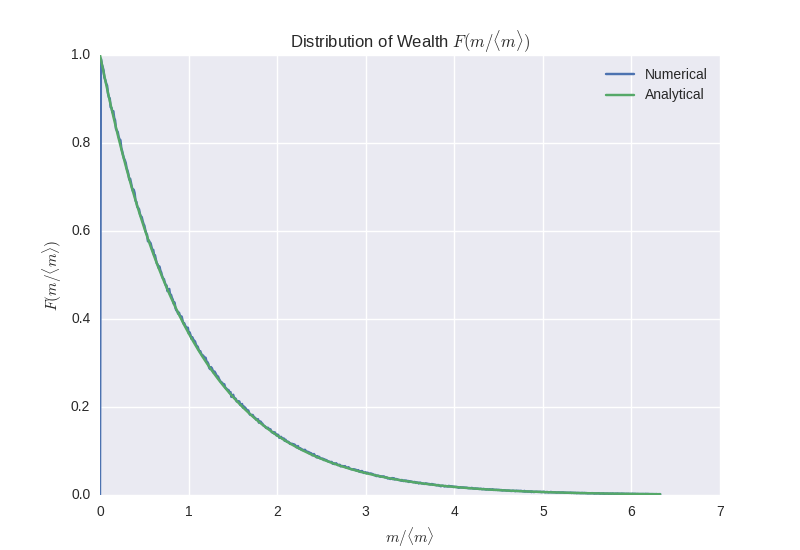
\includegraphics[height=2.5in]{distLamb0WAnalyt.png} %FIX THIS
\caption{Plot of figure \ref{fig:ModelA_final_distribution} together with the analytic solution from section \ref{Analytic_solution}}\label{fig:ModelA_final_distribution_with_analytic}
\end{figure}
\newpage
\subsubsection{Investigating the tail of the distribution from model A}
We also present a power law fit to the tail of our distribution, including both the numeric data, the analytic data and a power law fit applied to the tail of the numeric data. We discuss in section \ref{Tail_section} how we choose this tail. The plot is shown below:
\begin{figure}[!ht]
\centering
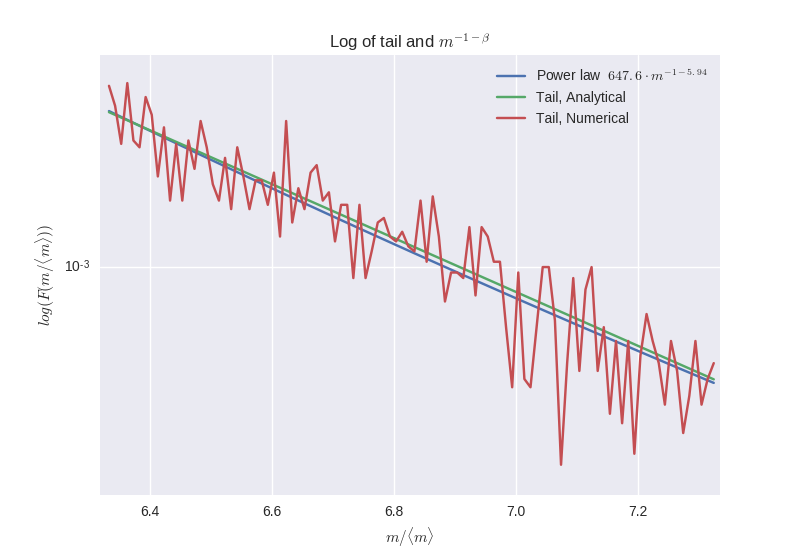
\includegraphics[height=2.5in]{tailPowerlamb0.png} %FIX THIS
\caption{The tail of the distribution from figure \ref{fig:ModelA_final_distribution}, together with a power law fit and the analytic solution.}\label{fig:ModelA_tail}
\end{figure}
\subsection{Discussion of model A}
\subsubsection{Choosing parameters}
As seen in figure \ref{fig:ModelA_Var}, the variance from a single run stabilizes after a few thousand interactions for this model. Note that this will, in general, depend upon the number of agents, as we need to ensure that every agent performs approximately the same number of transactions to get good statistical data. In our case, we have 500 agents. We therefore choose to perform $10^4$ Monte Carlo cycles, as we can see that the variance has stabilized at this point. This gives an average of 40 transactions per agent (as every transaction involves two agents), which should ensure that every agent is involved in at least a few transactions.\\
\linebreak
Figure \ref{fig:ModelA_MC_steps} shows the difference in the distribution between two successive Monte Carlo steps, as described by equation \ref{eq:Relative_diff_MC_steps}. For the first few cycles (not shown) this difference is very large (a difference of up to 35), but it quickly falls. We can see that the difference between two successive cycles quickly approaches zero. We choose $10^4$ Monte Carlo cycles as our cutoff point, where the relative difference is small enough to be essentially zero, but our simulations still run very quickly.
\subsubsection{The distribution}
As can be seen in figure \ref{fig:ModelA_final_distribution_with_analytic}, the analytic model agrees excellently with our simulations. The only exception is the very beginning: far fewer people have no wealth than predicted by the analytic model. This is not particularly surprising, however. The amount of wealth given to each agent at each transaction in this model depends on the number $\epsilon$, which is a floating point number in the interval $[0,1]$. Note, however, that the probability of $\epsilon$ being either exactly zero or exactly 1 is infinitesimal as these are floating point numbers. For an agent to end up with no wealth after a transaction, $\epsilon$ has to be one of these extreme values. Therefore, there are no agents with zero wealth, and this explains the dip at the very first data point. Closer inspection reveals that this dip is indeed only at the data point corresponding to 0 wealth.
\subsubsection{The tail of the distribution}
As can be seen in figure \ref{fig:ModelA_tail}, a power law fits the data fairly well. Note that there are significant oscillations in the data, even for many Monte Carlo steps, which are due to the lack of data at the high end of the tail (few people are very rich). Nonetheless, the trend is clear, and the power law hits the analytic solution rather well. Whilst it might be possible to decrease the oscillations in the data by increasing the number of Monte Carlo steps, this does not seems necessary, as the trend is present in the data. This shows that our model is fairly realistic, as it follows the empiric result of a Pareto distribution. The power law also reflects the analytic solution well.

\subsection{Results from the first modification (model B)}
\subsubsection{Results from our investigation into the optimal combination of parameters}
The results from our investigation into the optimal parameters for model B are shown below. We look at $\lambda \in [0,0.25, 0.5, 0.9]$. To determine the optimal parameters, however, we only include the plots for $\lambda = 0.9$ (the largest value of $\lambda$) as this value of $\lambda$ displayed the largest fluctuations.
\begin{figure}[!ht] %Fix this figure
    \centering
    \begin{subfigure}[H!]{0.5\textwidth}
        \centering
        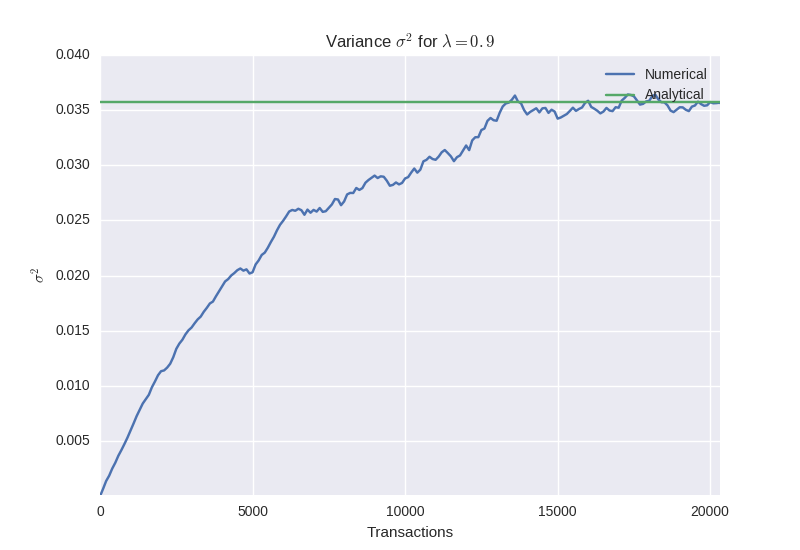
\includegraphics[height=2.0in]{varLamb09.png} %MAX VARIANCE
        \caption{The variance of a single Monte Carlo cycle in model B for $\lambda = 0.9$}\label{fig:ModelB_Var}
    \end{subfigure}%
    ~ 
    \begin{subfigure}[H!]{0.5\textwidth}
        \centering
        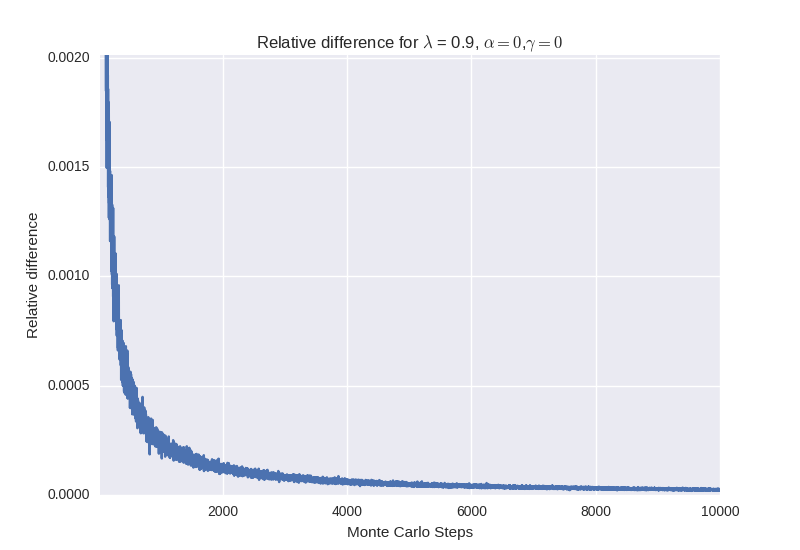
\includegraphics[height=2.0in]{relDiffL09A0G0.png}
        \caption{The relative difference in the distribution for successive Monte Carlo steps in model B, for $\lambda = 0.9$}\label{fig:ModelB_MC_steps}
    \end{subfigure}
    \caption{Plots from our investigation into the optimal choice of parameters in model B. Figure \ref{fig:ModelB_Var} shows how the variance the distribution for model B evolves with the number of transactions. This is for a single Monte Carlo cycle, with $N=500$ agents, and the initial wealth, $m_0=1000$. We have also included the analytic expression for this, derived in section \ref{Tail_section}. In figure \ref{fig:ModelB_MC_steps}, we show how the difference between successive average distributions evolves with the number of Monte Carlo steps. Each Monte Carlo step consists of $2\times 10^4$ transactions. Note that the $x$-axis does not start at zero, for a better graphical presentation of the long-term development.}\label{fig:ModelB}
\end{figure}
\newpage
\subsubsection{The distribution from model B}
We postpone a discussion of the choice of parameters until the discussion part later. We present the final, average, distribution, for this combination of parameters, below. We also include a logarithmic plot, similar to the one produced by \cite{Gibbs}.
\begin{figure}[!ht]
\centering
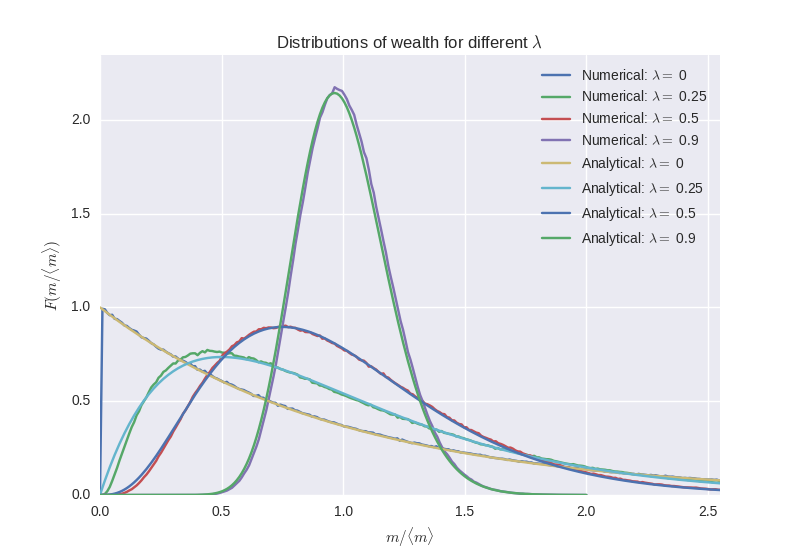
\includegraphics[height=2.5in]{distDiffLamb.png} %Fix this one
\caption{The final distribution of wealth from model B, for various values of $\lambda$. We also plot the analytic solution from section \ref{Analytic_solution}, to compare. Here $\langle m \rangle$ is the average wealth, which equals the initial wealth per agent, $m_0=1000$. This simulation was run with $500$ agents, performing $2\times 10^4$ transactions per Monte Carlo cycles, with a total of $10^4$ Monte Carlo cycles.}\label{fig:ModelB_final_distribution}
\end{figure}
\begin{figure}[!ht]
\centering
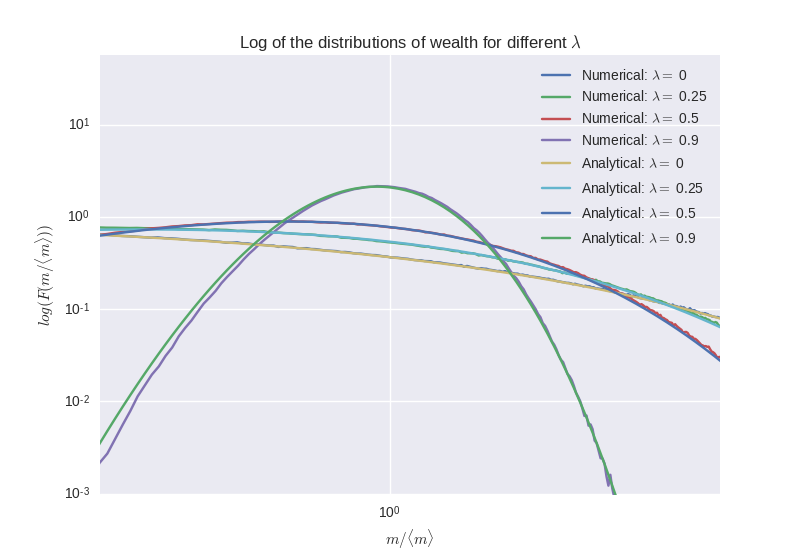
\includegraphics[height=2.5in]{logDistDiffLamb.png} %Fix this one
\caption{A logarithmic plot of figure \ref{fig:ModelB_final_distribution}}\label{fig:ModelB_final_distribution_log}
\end{figure}
\pagebreak
\subsubsection{Investigating the tail of the distribution from model B}
We also present a power law fit to the tail of our distribution, including both the numeric data, the analytic data and a power law fit applied to the tail of the numeric data. We discuss in section \ref{Tail_section} how we choose this tail. The plots, for our chosen values of $\lambda$, are shown below. Note that we have excluded the plot for $\lambda = 0$, as it is identical to figure \ref{fig:ModelA_tail}.
\begin{figure}[!ht] %Fix this figure
    \centering
    \begin{subfigure}[H!]{0.5\textwidth}
        \centering
        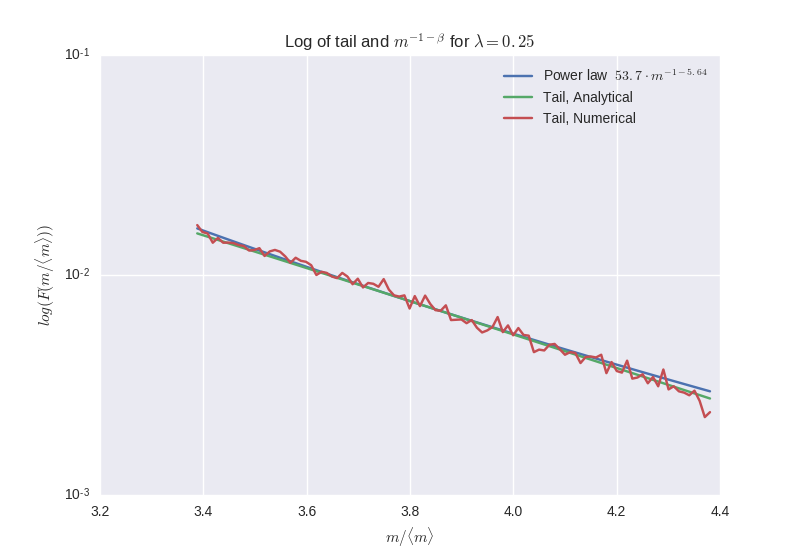
\includegraphics[height=2.0in]{tailPowerlamb025.png} %MAX VARIANCE
        \caption{$\lambda = 0.25$}\label{fig:ModelB_tail_lamb_025}
    \end{subfigure}%
    ~ 
    \begin{subfigure}[H!]{0.5\textwidth}
        \centering
        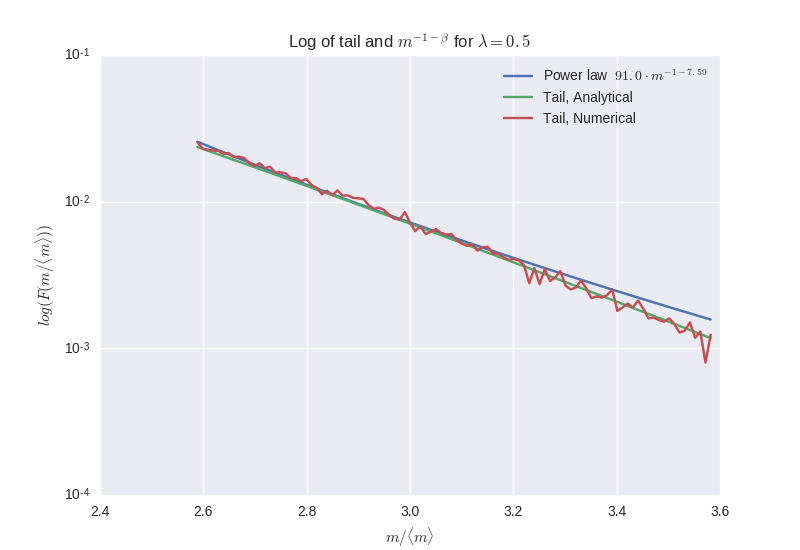
\includegraphics[height=2.0in]{tailPowerlamb05.png}
        \caption{$\lambda = 0.5$}\label{fig:ModelB_tail_lamb_05}
    \end{subfigure}
    \begin{subfigure}[H!]{0.5\textwidth}
        \centering
        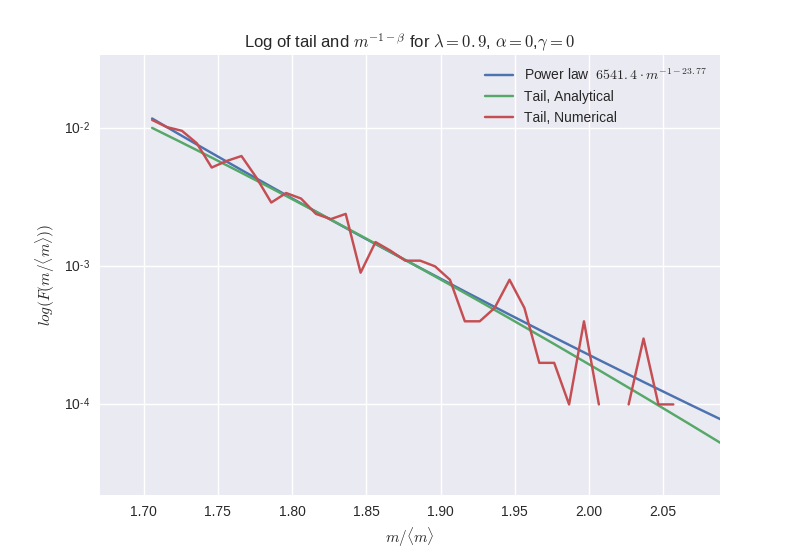
\includegraphics[height=2.0in]{tailL09A0G0_v2.png}
        \caption{$\lambda = 0.9$}\label{fig:ModelB_tail_lamb_09}
    \end{subfigure}
\caption{The tail of the distribution from figure \ref{fig:ModelB_final_distribution} (model B), together with a power law fit and the analytic solution from section \ref{Analytic_solution} for different values of $\lambda$.}\label{fig:ModelB_tail}
\end{figure} 

\subsection{Discussion of model B}
\subsubsection{Choosing parameters}
As can be seen in figure \ref{fig:ModelB_Var}, modifying the model by adding savings results in a longer equilibration time. In model A, $10^4$ transactions were more than sufficient to be safely inside equilibrium. This is not the case here. Therefore, we choose to double the number of transactions per Monte Carlo cycle, performing $2\times 10^4$ transactions per cycle. This should ensure that we are well inside equilibrium. Looking at figure \ref{fig:ModelB_MC_steps}, we see that $10^4$ Monte Carlo cycles again ensures that we are well inside equilibrium. Therefore, we again choose to perform $10^4$ Monte Carlo cycles.
\newpage
\subsubsection{The distribution}
The distribution for our chosen values of $\lambda$ is shown, together with the analytic solution, in figure \ref{fig:ModelB_final_distribution} and \ref{fig:ModelB_final_distribution_log}. Note that the distribution for $\lambda=0$ is identical to model A. For higher values of $\lambda$, the distribution appears to transition from a Gibbs distribution to something that resembles a normal distribution.\\
\linebreak
Large $\lambda$ implies that the amount of money exchanged at every time step is small. If this is the case, then each transaction results in small differences between players. Therefore, it is difficult to accumulate large amounts of wealth, as every transaction increases or decrease wealth by a small amount. For low values of $\lambda$, however, large amounts of money are exchanged at every time step. Note that, once wealth accumulates with a single agent, the subsequent interaction with this agent will again result in one of the agents having a large amount of wealth. Therefore, the distribution will tend to accumulate wealth with a few agents, leaving the rest relatively poor.\\
\linebreak
An alternative way to view this result is to realize that $\lambda=1$ corresponds to a uniform distribution (the initial distribution), whereas $\lambda=0$ corresponds to model A (Gibbs distribution). Thus, the values of $\lambda$ between these extremes, will vary between these points. This is what we observe; for low $\lambda$, the distribution is approximately equal to the Gibbs distribution from model A. For high $\lambda$, the distribution is more uniform. \\
\linebreak
Note, finally, that our figure \ref{fig:ModelC_final_distribution_log} correspond well with figure 2 presented in \cite{Gibbs}.
\subsubsection{The tail of the distribution}
In figure \ref{fig:ModelB_tail}, we present the tail of our distribution, together with the analytic solution and our power fit. Note that the fit works well for low values of $\lambda$, but less well for higher values. This is not particularly surprising. For low values of $\lambda$, there are more people with large amounts of wealth. Therefore, there is simply more data at the tail. Note that we have shifted the position of the tail slightly, but even so, there is little data for higher $\lambda$, as the transition into the more uniform distribution is pronounced. Nonetheless, the analytic solution clearly indicates that a power law should exist, if we had more data. Therefore, this model also seems to fit well with the assumption that the high-end distribution 
\newpage
\subsection{Results from the second modification (model C)}
\subsubsection{Results from our investigation into the optimal combination of parameters}
Here, we investigate $\alpha \in [0.5, 1.0, 1.5, 2.0]$, with $\lambda=0$. We present the variance for the two highest $\alpha$ below, as these showed the largest fluctuations.\\
\linebreak
\begin{figure}[!ht] %Fix this figure
    \centering
    \begin{subfigure}[H!]{0.5\textwidth}
        \centering
        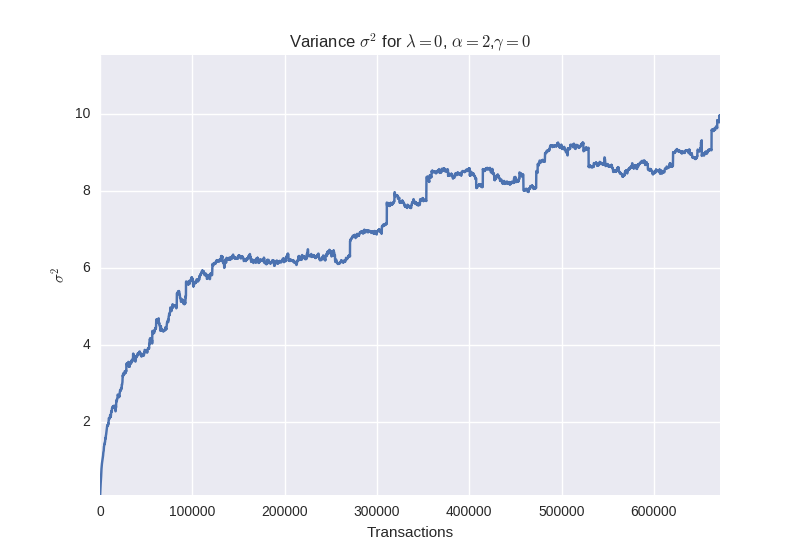
\includegraphics[height=2.0in]{varL0A2G0.png}
        \caption{$\alpha=2.0$}\label{fig:ModelC_Var_alpha_2}
    \end{subfigure}%
    ~ 
    \begin{subfigure}[H!]{0.5\textwidth}
        \centering
        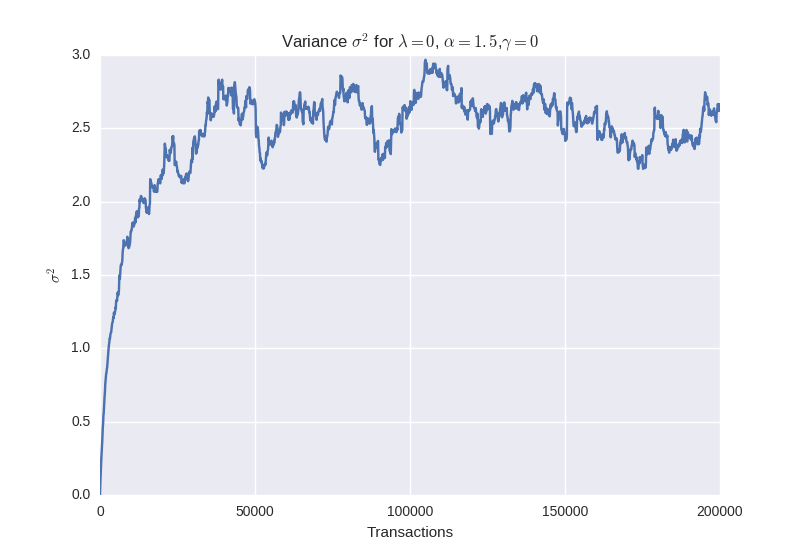
\includegraphics[height=2.0in]{varL0A15G0.png}
        \caption{$\alpha=1.5$}\label{fig:ModelC_Var_alpha_15}
    \end{subfigure}
    \caption{Plot of the variance for two different values of $\alpha$. This is for a single Monte Carlo cycle, with $N=1000$ agents, and initial wealth, $m_0=1000$}\label{fig:ModelC_variance}
\end{figure}
\linebreak
We also present how the distribution varies with successive Monte Carlo steps below. We show this only for $\alpha=2.0$, as this showed the largest deviation.
\begin{figure}[!hb]
\centering
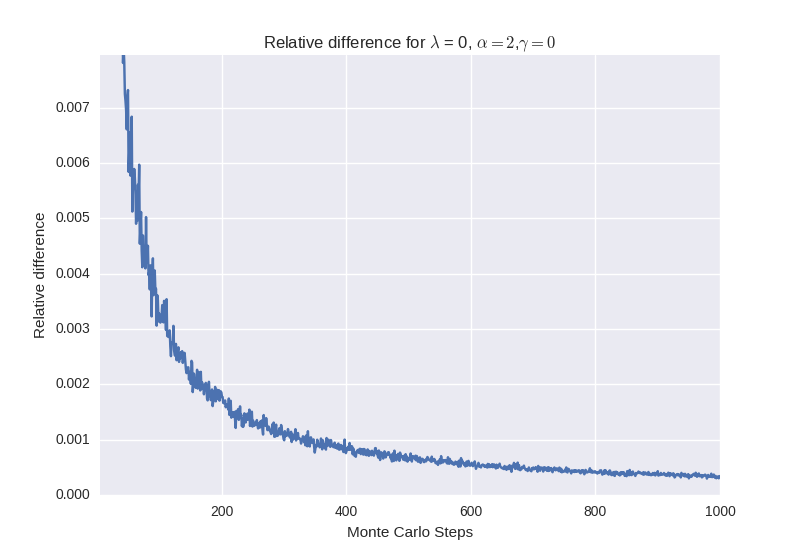
\includegraphics[height=2.5in]{relDiffL0A2G0.png} %Fix this one
\caption{The difference between successive average distributions as a function of the number of Monte Carlo steps. Each Monte Carlo step consists of $2\times 10^5$ transactions.}\label{fig:ModelC_MC_Steps}
\end{figure}
\newpage
\subsubsection{The distribution from model C}
Once again, the discussion of the choice of parameters is postponed until later. We present the final, average, distribution, for our values of $\alpha$, below, together with a log-log plot.
\begin{figure}[!ht]
\centering
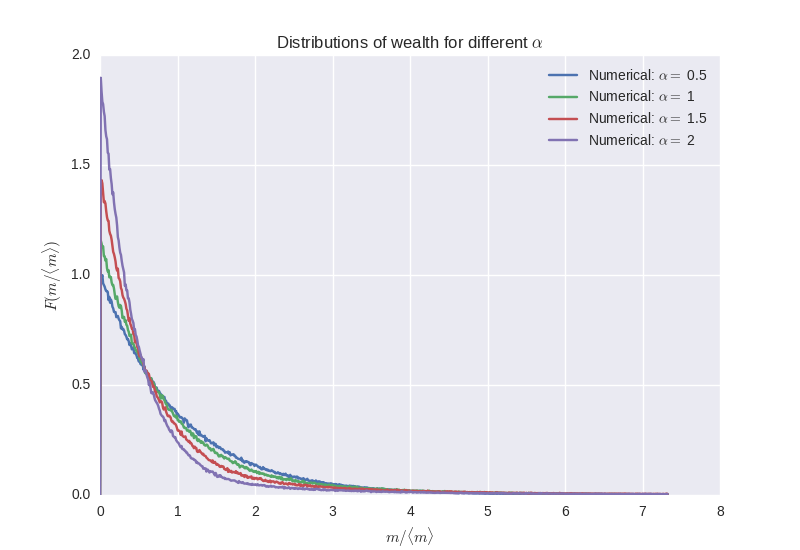
\includegraphics[height=2.5in]{distAlphas.png} %Fix this one
\caption{The final distribution of wealth from model C. Here $\langle m \rangle$ is the average wealth, which equals the initial wealth per agent, $m_0=1000$. This simulation was run with $1000$ agents, with $2 \times 10^5$ transactions per Monte Carlo cycles, for a total of $10^3$ Monte Carlo cycles.}\label{fig:ModelC_final_distribution}
\end{figure}
\begin{figure}[!ht]
\centering
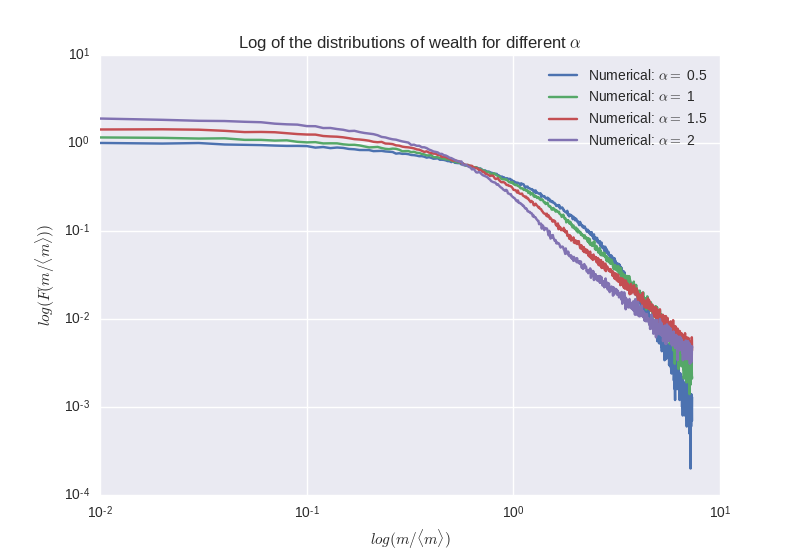
\includegraphics[height=2.5in]{logDistAlphas.png} %Fix this one
\caption{A log-log plot of figure \ref{fig:ModelC_final_distribution}}\label{fig:ModelC_final_distribution_log}
\end{figure}
\newpage
\subsubsection{Investigating the tail of the distribution from model C}
We also present a power law fit to the tail of our distribution. We discuss in section \ref{Tail_section} how we choose this tail. The plots, for our chosen values of $\alpha$ are shown below, together with the squared error in the power fit:
\begin{figure}[!ht] %Fix this figure
    \begin{subfigure}[H!]{0.5\textwidth}
        \centering
        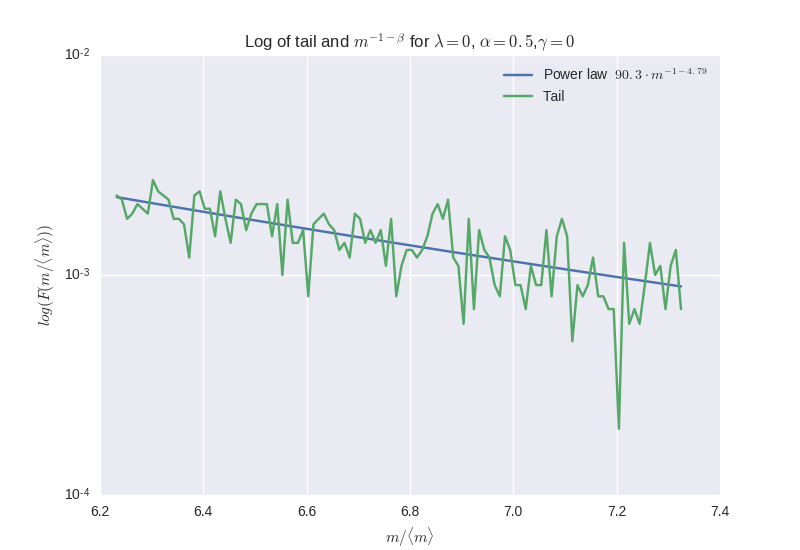
\includegraphics[height=2.0in]{tailL0A05G0.png} %MAX VARIANCE
        \caption{$\alpha = 0.5$}
    \end{subfigure}%
    ~ 
    \begin{subfigure}[H!]{0.5\textwidth}
        \centering
        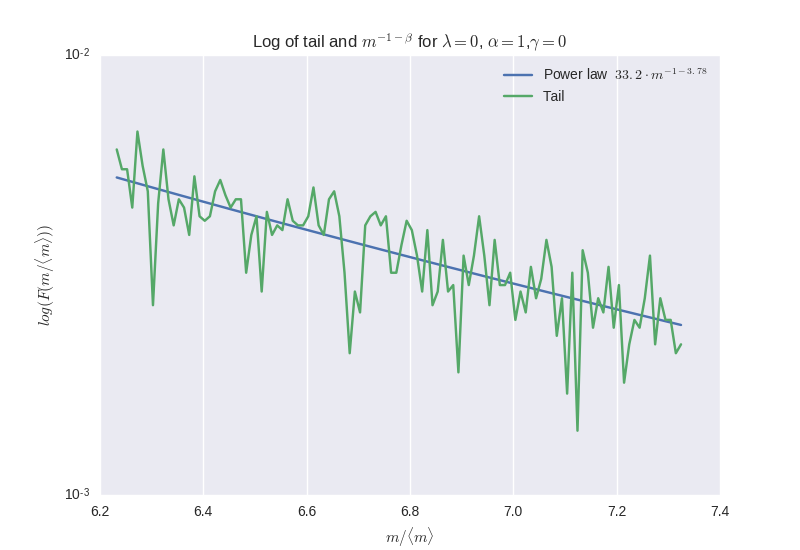
\includegraphics[height=2.0in]{tailL0A1G0.png}
        \caption{$\alpha = 1.0$}
    \end{subfigure}
     ~
    \begin{subfigure}[H!]{0.5\textwidth}
        \centering
        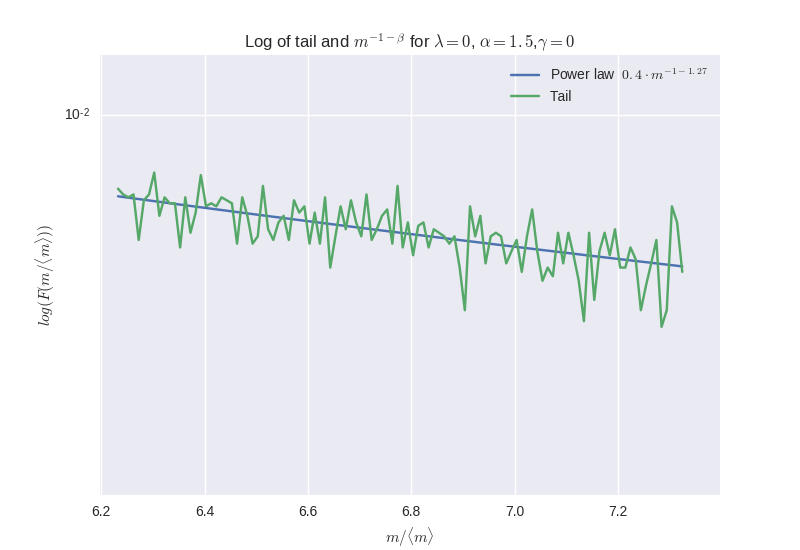
\includegraphics[height=2.0in]{tailL0A15G0.png}
        \caption{$\alpha = 1.5$}
    \end{subfigure}
     ~
    \begin{subfigure}[H!]{0.5\textwidth}
        \centering
        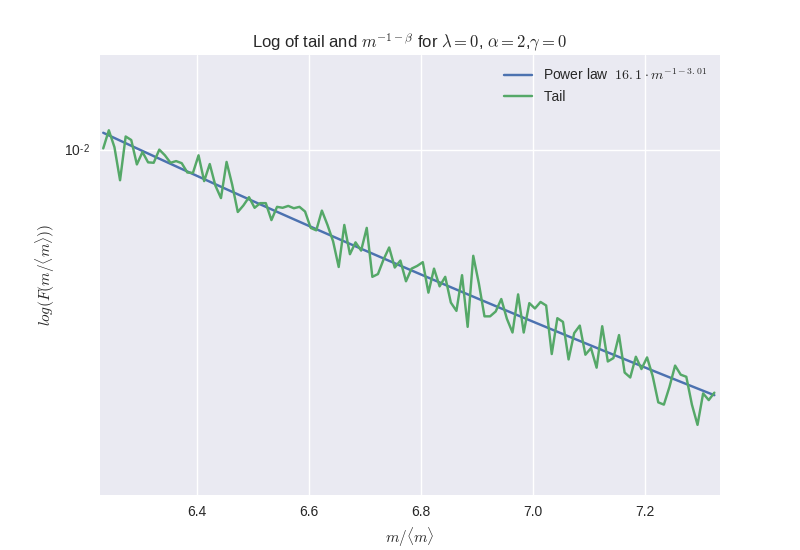
\includegraphics[height=2.0in]{tailL0A2G0.png}
        \caption{$\alpha = 2.0$}
    \end{subfigure}
\caption{The tail of the distribution from figure \ref{fig:ModelC_final_distribution} (model C), together with a power law fit.}\label{fig:ModelC_tail}
\end{figure} 
\begin{table}[!hb]
\centering
\caption{The squared error of the power law fit for different $\alpha$}\label{tab:Parameters_C}
\begin{tabular}{|c|c|}
\hline
$\alpha$ & Squared error\\
\hline
0.5& $1.40 \times 10^{-5}$\\
1& $4.40 \times 10^{-5}$\\
1.5 & $4.32 \times 10^{-5}$\\
2& $4.59\times 10^{-5}$\\
\hline
\end{tabular}
\end{table}
\newpage
\subsection{Discussion of model C}
\subsubsection{Choosing parameters}
As shown in figure \ref{fig:ModelC_Var_alpha_15} and \ref{fig:ModelC_Var_alpha_2}, the variance stabilizes very slowly, compared to the earlier models. There is a significant difference between $\alpha=1.5$ and $\alpha=2.0$, as $\alpha=2.0$ takes significantly longer to stabilize. Due to time constraints, and to maintain computational efficiency, we therefore decided to run $2\times 10^5$ transactions per Monte Carlo cycle. Note that this will not hit equilibrium for $\alpha=2.0$, but it will hit equilibrium for all other values of $\alpha$.\\
\linebreak
Figure \ref{fig:ModelC_MC_Steps} shows how the relative difference in the distribution varies with Monte Carlo cycles. Due to computational constraints, we were only able to produce this up to $10^3$ cycles. However,as the plot shows, the relative difference between successive cycles at this point is less than $0.001$. Therefore, we choose to employ $10^3$ cycles, to maintain computational efficiency. Note that this also indicates that the data for $\alpha=2.0$ are stable, and therefore reliable, despite not being at equilibrium.\\
\linebreak
Finally, we have decided to change our number of agents, $N$ to 1000, to more closely reflect the parameters chosen in \cite{AgentBased}.
\subsubsection{The distribution}
Figure \ref{fig:ModelC_final_distribution} shows the distribution for this model. This resembles our initial Boltzmann distribution for low values of $\alpha$. As $\alpha$ increases, however, the distributions become even more skewed - the tail of the distribution moves outwards (there are richer people), and the peak of the distribution increases (there are more poor people). This makes sense; low values of $\alpha$ will have relatively little impact on the distribution. As $\lambda=0$, this will then simply reproduce model A. For higher values of $\alpha$, the distribution changes significantly. Whenever two rich people interact, there is a significant probability that one of them will become much richer, and the other much poorer (depending on the value of $\epsilon$). We bias these interactions, so that the probability of a rich person interacting with a rich person increases significantly, and the probability of a poor person interacting with a poor person increases. Note that wealth only ever gets less concentrated if a rich and a poor person meet, and $\epsilon$ is close to 0.5. By making these interactions \textit{very} unlikely, we have significantly biased the system towards interactions which concentrate wealth on a single agent. This explains the observed distribution rather well. Notice also how the distribution for $\alpha=2.0$ follows this trend, despite not being entirely at equilibrium. This indicates that the lack of equilibrium is not a significant problem. Figure \ref{fig:ModelC_final_distribution_log} also resembles figure 1 in \cite{AgentBased}, which is reassuring.
\subsubsection{The tail of the distribution}
Figure \ref{fig:ModelC_tail} show the tail of the distribution, using a cut-off point discussed in section \ref{Tail_section}, and table \ref{tab:Parameters_C} summarizes the square error. Notice how there is a clear power law trend in all of these tails. This indicates that the model, at the very least, is consistent with a Pareto distribution at higher income.
\newpage
\subsection{Results from the final modification (model D)}
\subsubsection{Results from our investigation into the optimal combination of parameters}
The results from our investigation into the optimal parameters for model D are shown below. We include the plot for $\lambda = 0$, $\alpha=2$ and $\gamma=1$, as this took a significant amount of time to stabilize.
\begin{figure}[!ht]
    \centering
    \begin{subfigure}[H!]{0.5\textwidth}
        \centering
        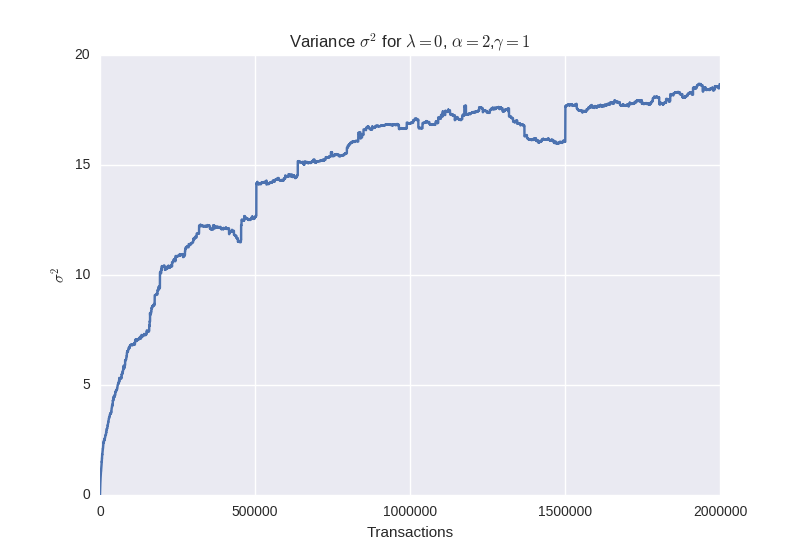
\includegraphics[height=2.0in]{varL0A2G1.png}
        \caption{The variance of a single Monte Carlo cycle}\label{fig:ModelD_var}
    \end{subfigure}%
    ~ 
    \begin{subfigure}[H!]{0.5\textwidth}
        \centering
        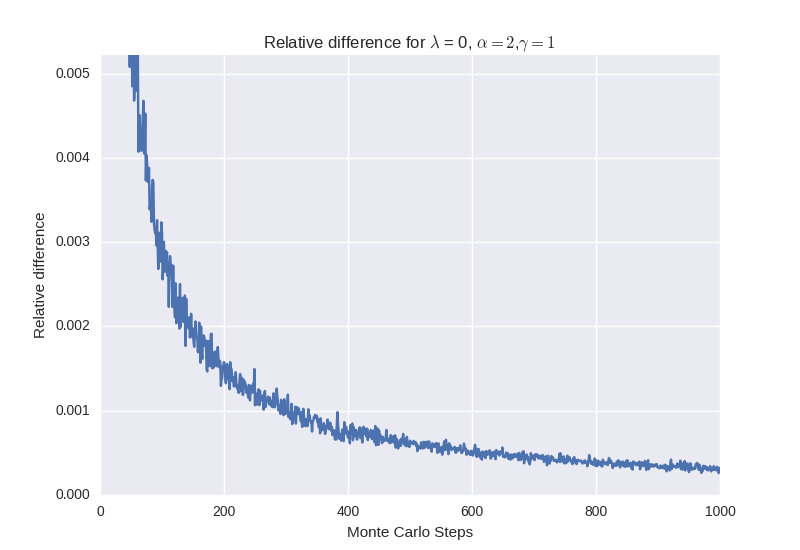
\includegraphics[height=2.0in]{relDiffL0A2G1.png}
        \caption{The difference in the distribution for successive Monte Carlo steps}\label{fig:ModelD_MC_steps}
    \end{subfigure}
    \caption{Plots from our investigation into the optimal choice of parameters, with $\lambda = 0$, $\alpha=2$ and $\gamma=1$. Figure \ref{fig:ModelD_var} shows how the variance of our distribution evolves with the number of transactions. This is for a single Monte Carlo cycle, with $N=1000$ agents, and initial wealth, $m_0=1000$. In figure \ref{fig:ModelD_MC_steps}, we show how the difference between successive average distributions evolves with the number of Monte Carlo steps. Each Monte Carlo cycles consists of $2\times 10^5$ transactions.}\label{fig:ModelD_parameters}
\end{figure} %ASK DANIEL ABOUT m0
\newpage
\subsubsection{The distribution from model D}
We postpone a discussion of the choice of parameters until the discussion part later. We present the final, average, distribution, for this combination of parameters, below, once again together with a logarithmic plot:
\begin{figure}[!hb] %Fix this figure
	\centering
    \begin{subfigure}[H!]{0.5\textwidth}
    	\centering
    	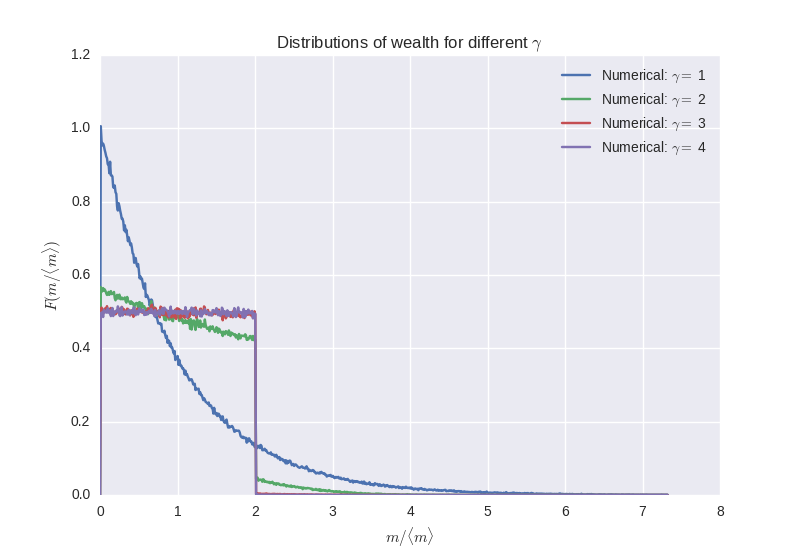
\includegraphics[height=2.0in]{distGammasA0.png}
    	\caption{$\alpha = 0$, $\lambda=0$}\label{fig:ModelD_dist_1}
    \end{subfigure}%
    ~
    \begin{subfigure}[H!]{0.5\textwidth}
        \centering
        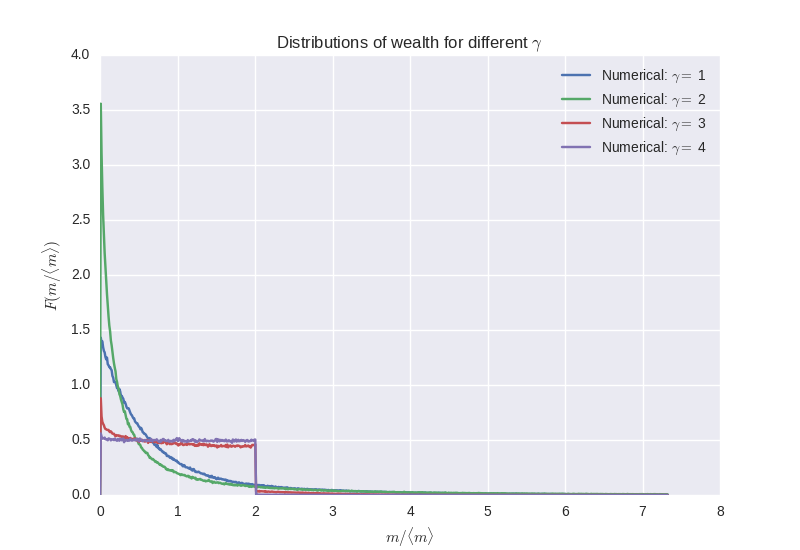
\includegraphics[height=2.0in]{distGammasA1.png} %MAX VARIANCE
        \caption{$\alpha = 1$, $\lambda=0$}\label{fig:ModelD_dist_2}
    \end{subfigure}
    ~ 
     \begin{subfigure}[H!]{0.5\textwidth}
        \centering
        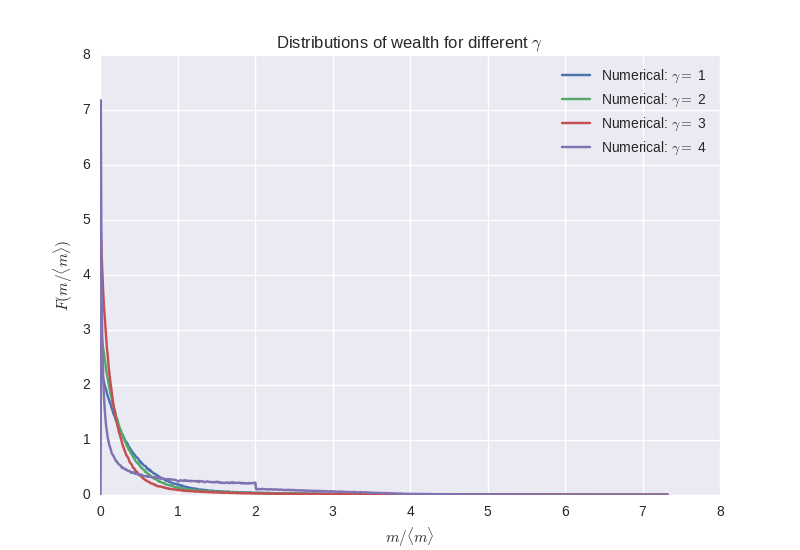
\includegraphics[height=2.0in]{distGammasA2.png}
        \caption{$\alpha = 2.0$, $\lambda=0$}\label{fig:ModelD_dist_3}
    \end{subfigure}%
    ~
       \begin{subfigure}[H!]{0.5\textwidth}
        \centering
        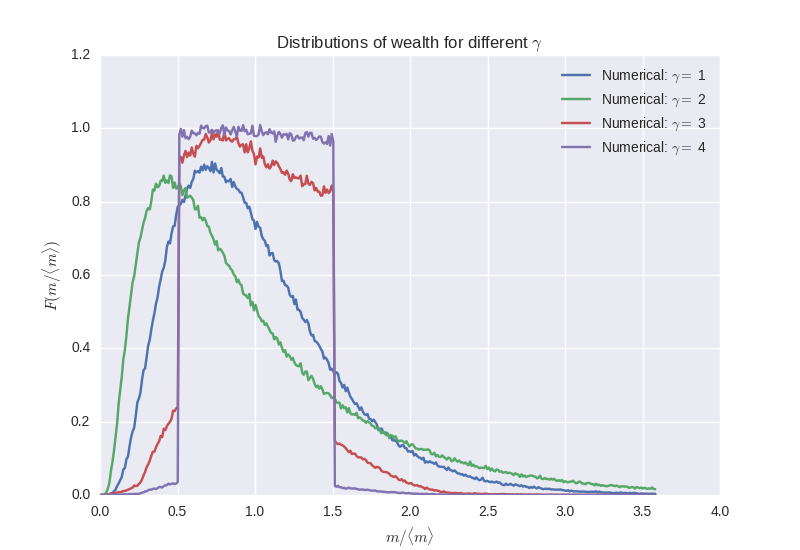
\includegraphics[height=2.0in]{distGammasA1L05.png}
        \caption{$\alpha = 1, \lambda=0.5$}\label{fig:ModelD_dist_4}
    \end{subfigure}
\caption{The distribution of model D for different parameter combinations. This was created with $N=1000$ agents, initial money, $m_0=1000$, using $10^3$ Monte Carlo cycles, each consisting of $2\times 10^5$ transactions.}\label{fig:ModelD_dist}
\end{figure}
\begin{figure}[!ht] %Fix this figure
	\centering
    \begin{subfigure}[H!]{0.5\textwidth}
    	\centering
    	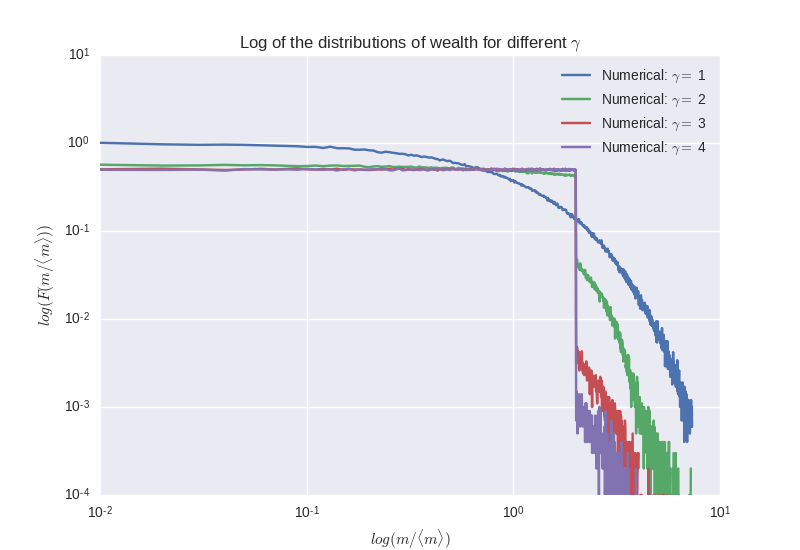
\includegraphics[height=2.0in]{logDistGammasA0.png}
    	\caption{$\alpha = 0$, $\lambda=0$}
    \end{subfigure}%
    ~
    \begin{subfigure}[H!]{0.5\textwidth}
        \centering
        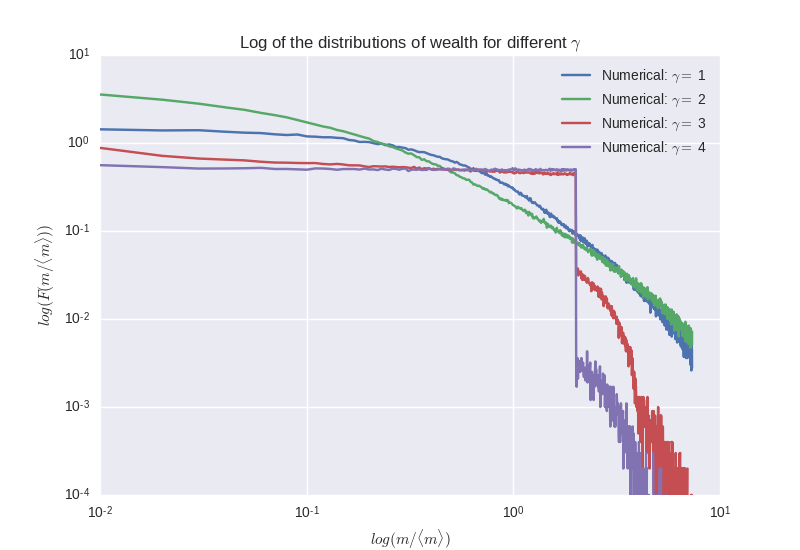
\includegraphics[height=2.0in]{logDistGammasA1.png} %MAX VARIANCE
        \caption{$\alpha = 1$, $\lambda=0$}\label{fig:ModelD_dist_1_log}
    \end{subfigure}
    ~ 
     \begin{subfigure}[H!]{0.5\textwidth}
        \centering
        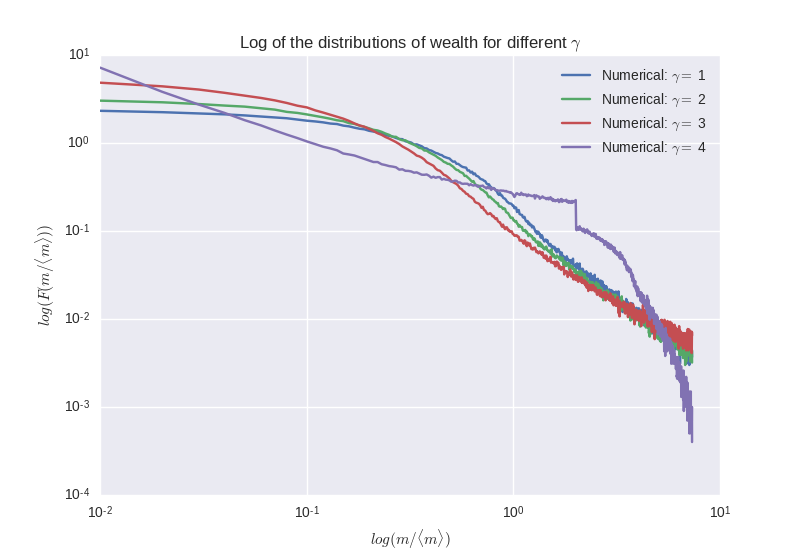
\includegraphics[height=2.0in]{logDistGammasA2.png}
        \caption{$\alpha = 2.0$, $\lambda=0$}
    \end{subfigure}%
    ~
       \begin{subfigure}[H!]{0.5\textwidth}
        \centering
        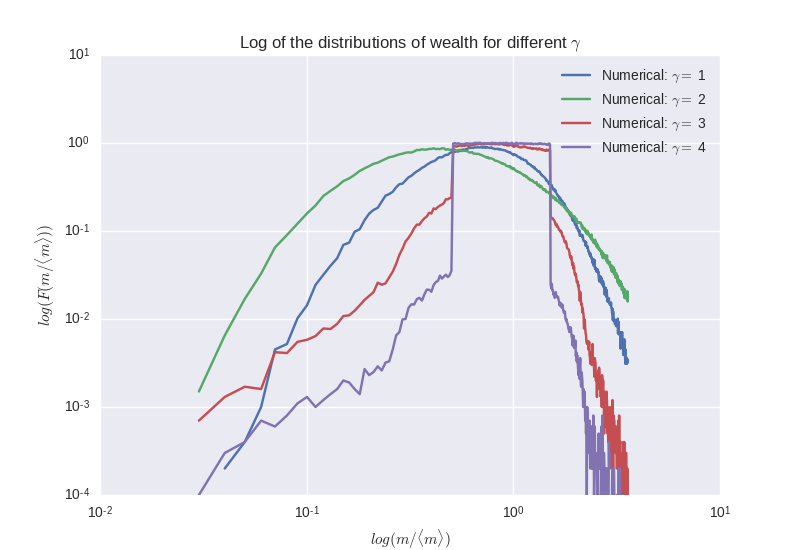
\includegraphics[height=2.0in]{logDistGammasA1L05.png}
        \caption{$\alpha = 1, \lambda=0.5$}
    \end{subfigure}
\caption{Log-log plot of figure \ref{fig:ModelD_dist}} \label{fig:ModelD_dist_log}
\end{figure}
\newpage
\subsubsection{Investigating the tail of the distribution from model D}
We also present a power law fit to the tail of our distribution, including the numeric data, together with the squared error of the fit. We discuss in section \ref{Tail_section} how we choose this tail. 
\begin{figure}[!ht] %Fix this figure
	\centering
    \begin{subfigure}[H!]{0.5\textwidth}
        \centering
        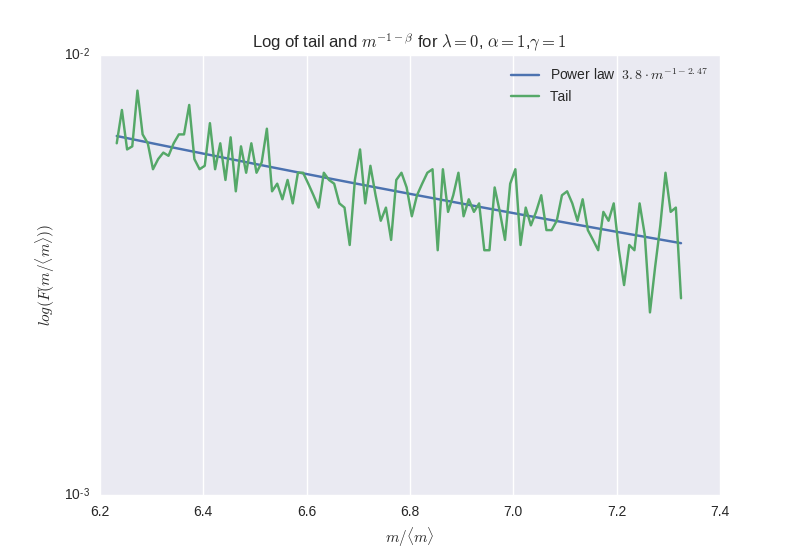
\includegraphics[height=2.0in]{tailL0A1G1.png} %MAX VARIANCE
        \caption{$\lambda=0, \alpha=1, \gamma = 0.5$}
    \end{subfigure}%
    ~ 
    \begin{subfigure}[H!]{0.5\textwidth}
        \centering
        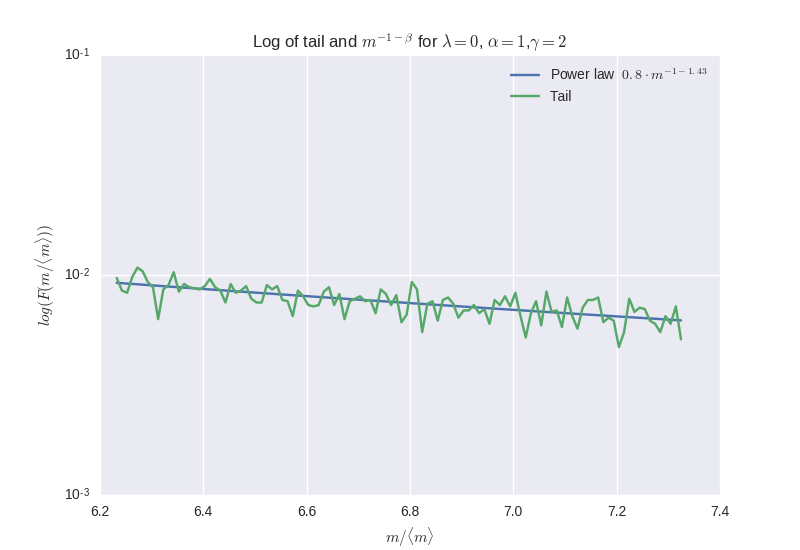
\includegraphics[height=2.0in]{tailL0A1G2.png}
        \caption{$\lambda = 0, \alpha = 1.0, \gamma=2.0$}
    \end{subfigure}
     ~
    \begin{subfigure}[H!]{0.5\textwidth}
        \centering
        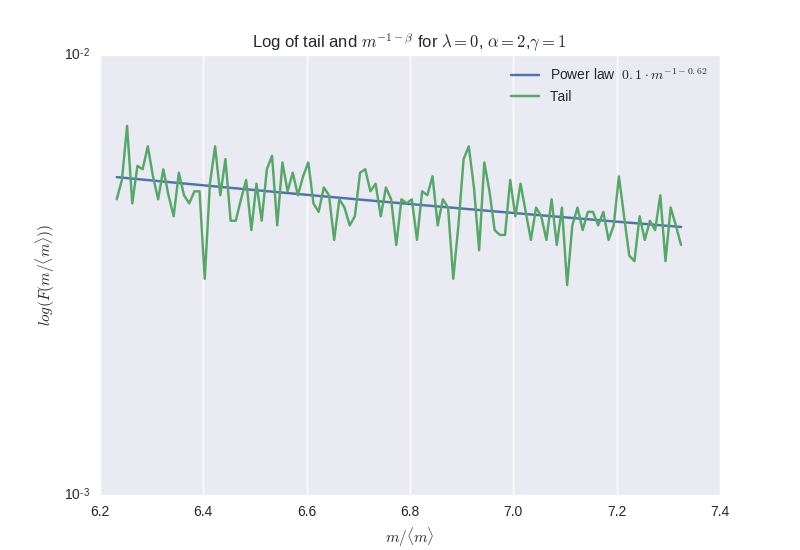
\includegraphics[height=2.0in]{tailL0A2G1.png}
        \caption{$\lambda=0, \alpha = 2, \gamma=1$}
    \end{subfigure}%
     ~
    \begin{subfigure}[H!]{0.5\textwidth}
        \centering
        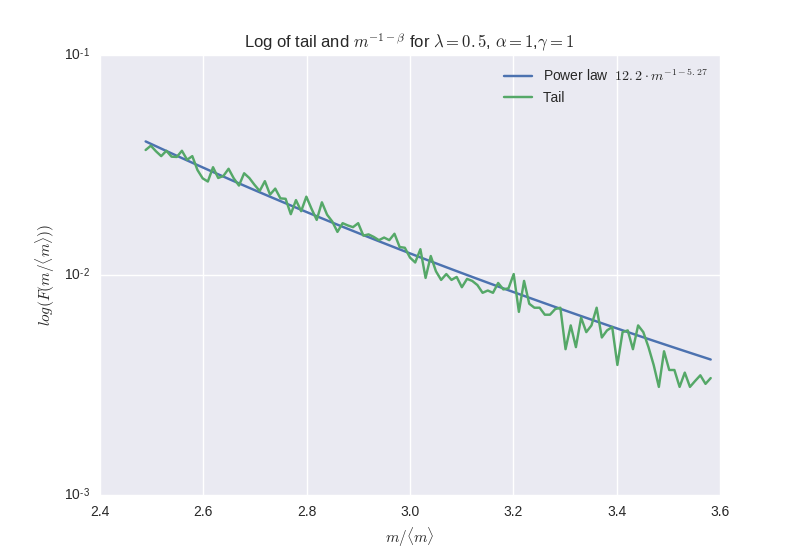
\includegraphics[height=2.0in]{tailL05A1G1.png}
        \caption{$\lambda=0.5, \alpha=1, \gamma=1$}
    \end{subfigure}
    ~
      \begin{subfigure}[H!]{0.5\textwidth}
        \centering
        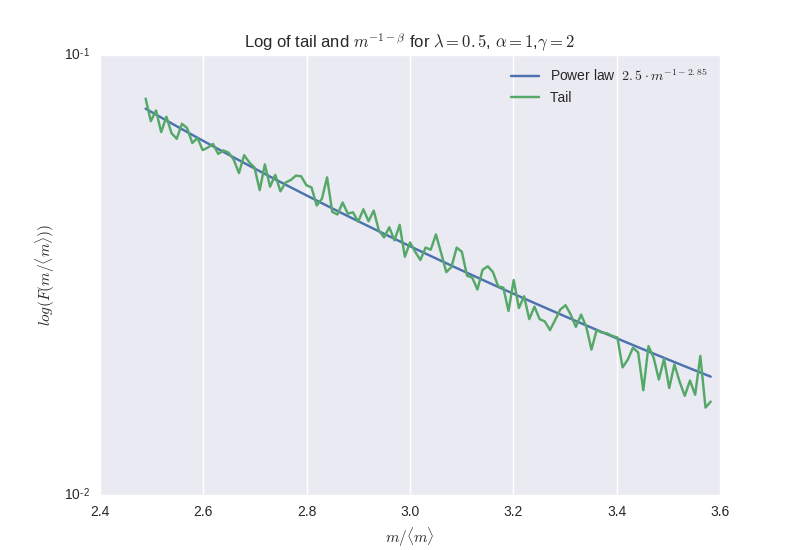
\includegraphics[height=2.0in]{tailL05A1G2.png}
        \caption{$\lambda=0.5, \alpha=1, \gamma=2$}
    \end{subfigure}
\caption{The tail of the distribution from figure \ref{fig:ModelD_dist} (model D), together with a power law fit.}\label{fig:ModelD_tail}
\end{figure}
\begin{table}[!hb]
\centering
\caption{Square error of power law fit for different combination of parameters}\label{tab:parameters_D}
\begin{tabular}{|c|c|c|c|}
\hline
$\lambda$ & $\alpha$ & $\gamma$ & Squared error\\
\hline
0 & 1 & 1 & $4.43\cdot 10^{-5}$\\
0 & 1 & 2 & $7.69\cdot 10^{-5}$\\
0 & 2 & 1 & $4.33\cdot 10^{-5}$\\
0 & 2 & 2 & $7.20 \cdot 10^{-5}$\\
0.5 & 1 & 1 & $2.22\cdot 10^{-4}$\\
0.5 & 1 & 2 & $5.62\cdot 10^{-4}$\\
\hline
\end{tabular}
\end{table} 
\clearpage
\subsection{Discussion of model D}
\subsubsection{Choosing parameters}
As can be seen in figure \ref{fig:ModelD_dist}, the variance once again takes a long time to stabilizes. Even after $2\times 10^6$ transactions, the equilibrium is still dubious. Therefore, we choose $2 \times 10^5$ transactions per Monte Carlo cycle. Notice how the relative difference between the distributions quickly vanishes even with just $2\times 10^5$ cycles. Therefore, if we choose $10^3$ Monte Carlo cycles, we can assume that we have reliable data. Whilst it is not equilibrium, it is at least stable. This is therefore the most viable alternative to equilibrium, given our strict time constraints. We once again chose $N=1000$ agents, to make comparison between model C and D more reliable. 

\subsubsection{The distribution}
Figure \ref{fig:ModelD_dist} shows the distribution for a variety of parameters. We begin by discussing figure \ref{fig:ModelD_dist_1}.\\
\linebreak
In figure \ref{fig:ModelD_dist_1}, we show purely the effect of the psychological propinquity factor $\gamma$, with $\alpha=0$ and $\lambda=0$. For $\gamma=1$, the effect seems rather small, as the shape is similar to the shape of model A, albeit somewhat more stretched. For $\gamma = 2$ and upwards, however,the distribution suddenly becomes discontinuous, seemingly at exactly twice the mean, splitting the population into a large group of poor to upper middle class and a very small fraction of rich people. There seems to be a rather sharp transition somewhere between $\gamma=1$ and $2$, which may indicate a sort of phase transition in the system. This is a very odd behavior, which must be analyzed in the context of the other results.\\
\linebreak
Figure \ref{fig:ModelD_dist_2} and \ref{fig:ModelD_dist_3} include the effect of economic closeness, through the parameters $\alpha$. Notice how this appears to delay the phase transition - for $\alpha=1$, the curves for $\gamma=1$ and $\gamma=2$ seem to follow the Boltzmann distribution which we observed for model C, whereas it again turns into a discontinuous distribution for higher $\gamma$. For $\alpha=2$, the phase transition is further delayed,until $\gamma=4$. This seems to indicate that there are two competing factor at play - that $\alpha$ and $\gamma$ counteract one another. These parameters determine the probability of an interaction happening. It seems that, if the probability of an interaction is given by the $\alpha$ term, the distribution will approximately follow a Gibbs distribution, whereas the distribution will approach something like a uniform distribution in two different regimes if $\gamma$ is large enough relative to $\alpha$ (and $\gamma$ is larger than unity).\\
\linebreak
Finally, consider figure \ref{fig:ModelD_dist_4}, where we also include the effect of saving. Note that the phase transition occurs at the same values for $\gamma$ as in figure \ref{fig:ModelD_dist_2}, which had the same $\alpha$. This indicates that $\lambda$ has little effect on the appearance of the phase transition. However, $\lambda$ drastically changes the shape of the phase transition. By introducing a $\lambda$, we narrow the distribution, and cause the peak to be in rather towards the middle. Note that the distribution for $\gamma < 3$  looks very similar to the distribution from model C. This supports the theory that $\gamma$ and $\alpha$ are somehow competing.\\
\linebreak
It is rather difficult to get an intuitive grasp of what is going on. One possible explanation, however, is this: note that, initially (after few transactions), $\gamma$ has little to say, as the factor containing $\gamma$ scales with the interactions. Thus initially, the $\alpha$ factor has to be dominating. As seen earlier, $\alpha$ tends to skew the distribution - so that very few people are extremely rich. Now the rich people will tend to only interact among themselves, whereas the poorer will tend to interact only among themselves. Thus, the correlation matrix, $c_{ij}$, constantly increases for people of comparable wealth. As we scale the $\gamma$ probability with the maximum of the $c_{ij}$ matrix, the probability of two people from different echelons of society interacting becomes utterly negligible. At some point (earlier if $\gamma$ is much larger than $\alpha$), $\gamma$ therefore dominates the interaction, favoring only interaction between people with similar wealth. From this it is not at all clear why the $\gamma$ distribution looks the way it looks however, nor why the discontinuity occurs at $2\langle m \rangle$. This also does not explain the shape of figure \ref{fig:ModelD_dist_4}.
\linebreak
One potential problem may be that we are not yet at equilibrium. What may be happening is that the $\gamma$  factor will always dominate after a long time, but that we do not simulate long enough for this to happen. If this is the case, then we may expect all distributions to approach this odd "stepping" behavior for enough transactions per Monte Carlo cycle. We therefore repeat some selected runs with as many transactions as our time frame allowed - which in this case was $10^6$ transactions per time step. We show the log-plot from this below, next to the original image:\\
\linebreak
\begin{figure}[!hb] %Fix this figure
    \begin{subfigure}[H!]{0.5\textwidth}
        \centering
        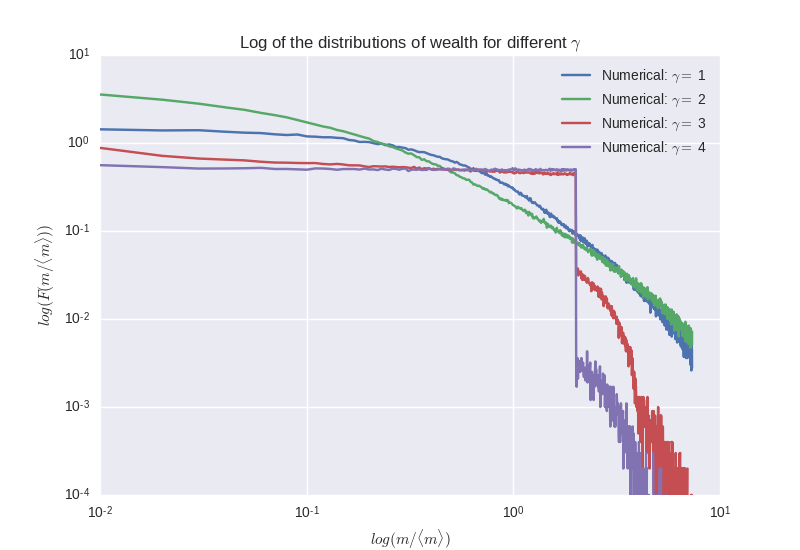
\includegraphics[height=2.0in]{logDistGammasA1.png} %MAX VARIANCE
        \caption{$\lambda=0, \alpha=1$, $\mathrm{Transactions/cycle}=2\times 10^5$}
    \end{subfigure}%
    ~ 
    \begin{subfigure}[H!]{0.5\textwidth}
        \centering
        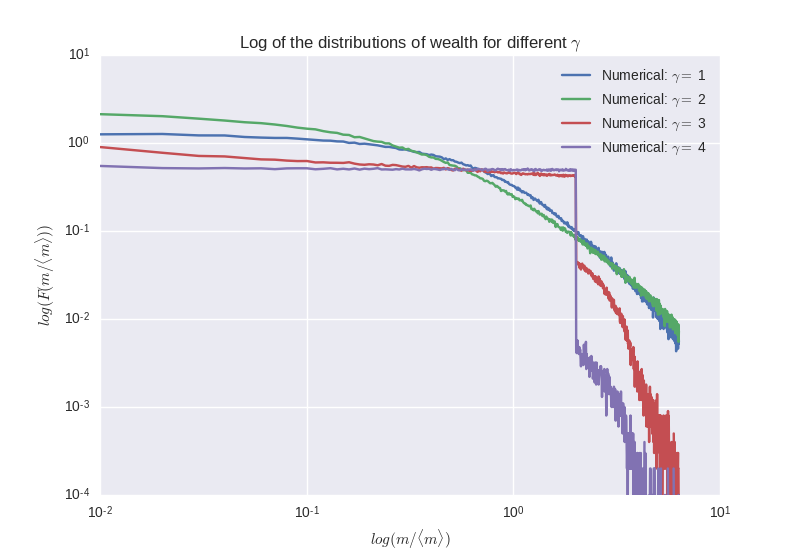
\includegraphics[height=2.0in]{logDistGammasA1_v2.png}
        \caption{$\lambda=0, \alpha=1$, $\mathrm{Transactions/cycle}= 10^6$}
    \end{subfigure}
     ~
    \begin{subfigure}[H!]{0.5\textwidth}
        \centering
        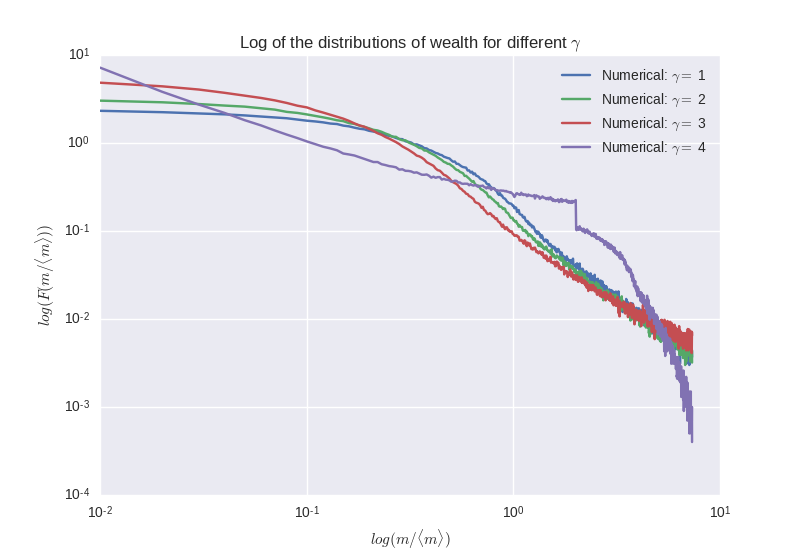
\includegraphics[height=2.0in]{logDistGammasA2.png}
        \caption{$\lambda=0, \alpha=2$, $\mathrm{Transactions/cycle}=2\times 10^5$}
    \end{subfigure}
     ~
    \begin{subfigure}[H!]{0.5\textwidth}
        \centering
        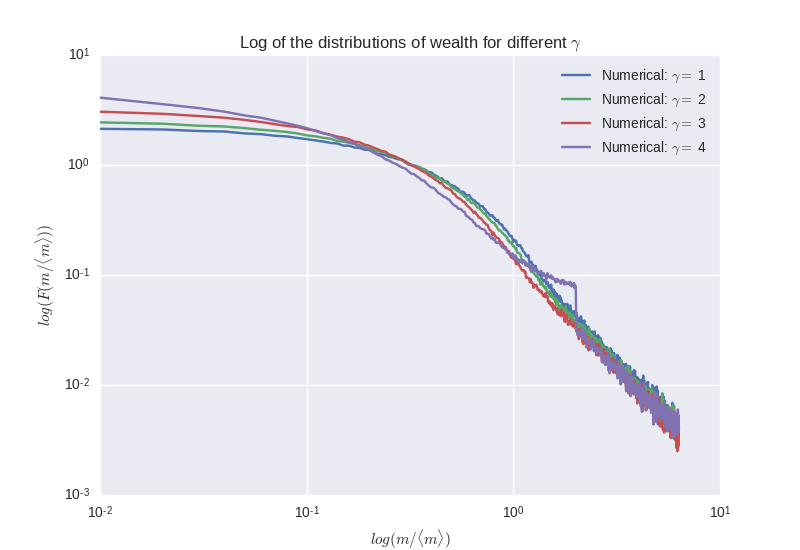
\includegraphics[height=2.0in]{logDistGammasA2_v2.png}
        \caption{$\lambda=0, \alpha=2$, $\mathrm{Transactions/cycle}=10^6$}
    \end{subfigure}
\caption{Some plots from figure \ref{fig:ModelD_dist_log}, together with a version with more transactions per Monte Carlo cycle}
\end{figure}
\linebreak
Note how the increasing the number of transactions by a factor 5 has barely changed the plot for $\alpha=2$, but has significantly changed the plot for $\alpha=2$. This indicates that we are further from equilibrium at higher $\alpha$, which supports the idea that $\gamma$ and $\alpha$ are competing factors. Note further, however, that no additional phase transitions are observed, and that the phase transitions for $\alpha=2$ seem to become less prominent with more transactions. There is therefore no indication of additional phase transitions occurring with more transactions - rather the opposite. Note further that we have not entirely managed to reproduce figure 5 in \cite{AgentBased}. Whilst it is not entirely clear what parameters were chosen in that article, the difference in slope is nonetheless striking. This may indicate that increasing time steps significantly may reveal additional behavior. Either way, there clearly remains a significant amount of research before this model is entirely understood.
\subsubsection{The tail of the distribution}
We show the tails for a variety of parameter combinations in figure \ref{fig:ModelD_tail}, with the errors in table \ref{tab:parameters_D}. Once again, the trend is convincing in all of these plots. This indicates that the tail of our models can be modelled as a Pareto distribution.  
\section{Conclusion}
\subsection{Conclusion}
We have investigated four different ways in which economic agents may wish to interact, using models developed by \cite{Gibbs} and \cite{AgentBased}. We have found good agreement with the available analytic solutions throughout, both for development of the variance of the distributions and for the distributions themselves. We have also found good agreement with the empirical fact that such distributions tend to follow a Pareto distribution at high incomes for all distribution.\\
\linebreak
We have been able to provide a working explanation for model A, B and C, which correspond well with what we observe. This was difficult with model D, as we observed some odd behavior. We were only partially able to explain the results from model D. This model therefore requires further research.
\subsection{Outlook}
The four models presented and investigated here are only a small sliver of the available models. In the future, it may be very interesting to implement additional modifications to these models. One exciting alternative is provided by \cite{DoublePower}, where interest rates are added to the economy - making the rich even richer. Additional potential modifications could include government intervention, inflation or collusion and the formation of oligopolies, to name a few.\\
\linebreak
It would also be interesting to further investigate the Pareto fits, and investigate if the exponent of these distributions can be linked to something physically meaningful in the models.\\
\linebreak
Finally, it would of course be interesting to further investigate model D, to try and understand the apparent phase transition - and whether or not this is a real effect or an error in our model. It would be interesting to significantly boost the number of transactions per Monte Carlo cycle, to see whether or not the phase transition always occur. It would also be interesting to observe exactly at which $\gamma$ the phase transition occurs, and whether or not this has a physical significance.
\newpage

\newpage
\addcontentsline{toc}{section}{References}
\bibliography{Project5Bib}
\bibliographystyle{apalike}

\end{document}

%%INCLUDE INITIAL MONEY